%*****************************************************A**************************
%********************************** Chapter XXXXXXXX ***************************
%*******************************************************************************

\nomenclature[z-MIP]{MIP}{Minimally Ionising Particle}
\nomenclature[z-MPV]{MPV}{Most Probable Value} 
\nomenclature[z-PID]{PID}{Particle IDentification}

\chapter{Simulations of the 35 ton prototype}  %Title of chapter

\graphicspath{{35tonSimulation/Figs/PDF/}{35tonSimulation/Figs/Raster/}{35tonSimulation/Figs/}}

%********************************** %First Section  *************************************
\section{Determination of interaction times} \label{sec:SimInteractionTimes} %Section - X.1
As outlined at the end of Section~\ref{sec:LArSoft} it is important to know the interaction time of a track when performing calorimetric reconstruction. When performing simulations the simplest interaction time to assign to a reconstructed object is the Monte Carlo truth time of when the particle was created. The creation time can be used as the distances considered in simulations are small compared to the velocities which the particles are initially travelling meaning that interactions throughout the volume are less than the resolution of the detector (500 ns). When matching a reconstructed object with a GEANT4 particle the particle which contributed the most overall deposited charge to the whole track is chosen. This means that the energy deposited for each hit on the track is broken down into how much each particle contributed to the charge of the individual hit, with the energies summed over all hits. The ability to assign the true interaction times to 3D objects is vital when wanting to benchmark how well other determinations of interaction times perform or to determine the efficiency of the tracking algorithms as described in Section~\ref{sec:SimRecoEffic}. \\

In the 35 ton detector, it was envisioned that there would be at least two ways in which interaction times could be assigned to tracks, one using the external cosmic ray counters and another using reconstructed scintillation light collected by the photon detectors. The cosmic ray counters were used extensively in the 35 ton data, as described in Section~\ref{sec:DataAlgs}, however in simulation the scintillation light was used as this would have been more powerful during continuous running as not all particles would pass through counters but one wold expect almost all of them to produce reconstructable scintillation light. Flashes of lights are reconstructed by using a prebuilt library which models the expected number of photoelectrons to be measured on each photon detector given the 3D position of the source of the flash. This library takes into account the expected quantum efficiencies of each photon detector. \\

When trying to produce an association metric a sample of 10,000 Anti-Muons with a cosmic-like distribution was used as then there there should only be one long track with which to match one reconstructed flash. A cosmic-like distribution is defined as a set of particles which have a $\cos^{2}$ angular distribution, no minimum or maximum energies and have a flat distrbution of initial positions in the $xz$ plane and a uniform initial $y$ position. When this sample was simulated it was clear that the photon detector reconstruction using the prebuilt libraries worked well as the reconstructed flash source normally lay very close to the track which caused it. It was found that a calculation of a Point Of Closest Approach (PoCA)!!~citep{PoCA}!! of the reconstructed track to the flash source gave an effective metric by which the two could be combined. Other metrics such as the distance between the flash source and the track centre, and the perpendicular distance between the flash source and the line joining the start and end of track were investigated but found to provide a less reliable metrics. The latter of these metrics is less effective because the reconstructed tracks are rarely straight lines, due to particles scattering as they travel through the LAr and so the perpendicular distance at each hit must be calculated. A comparison of these metrics is shown in Figure~\ref{fig:PDYZDist}. \\

\begin{figure}[h!]
  \centering
  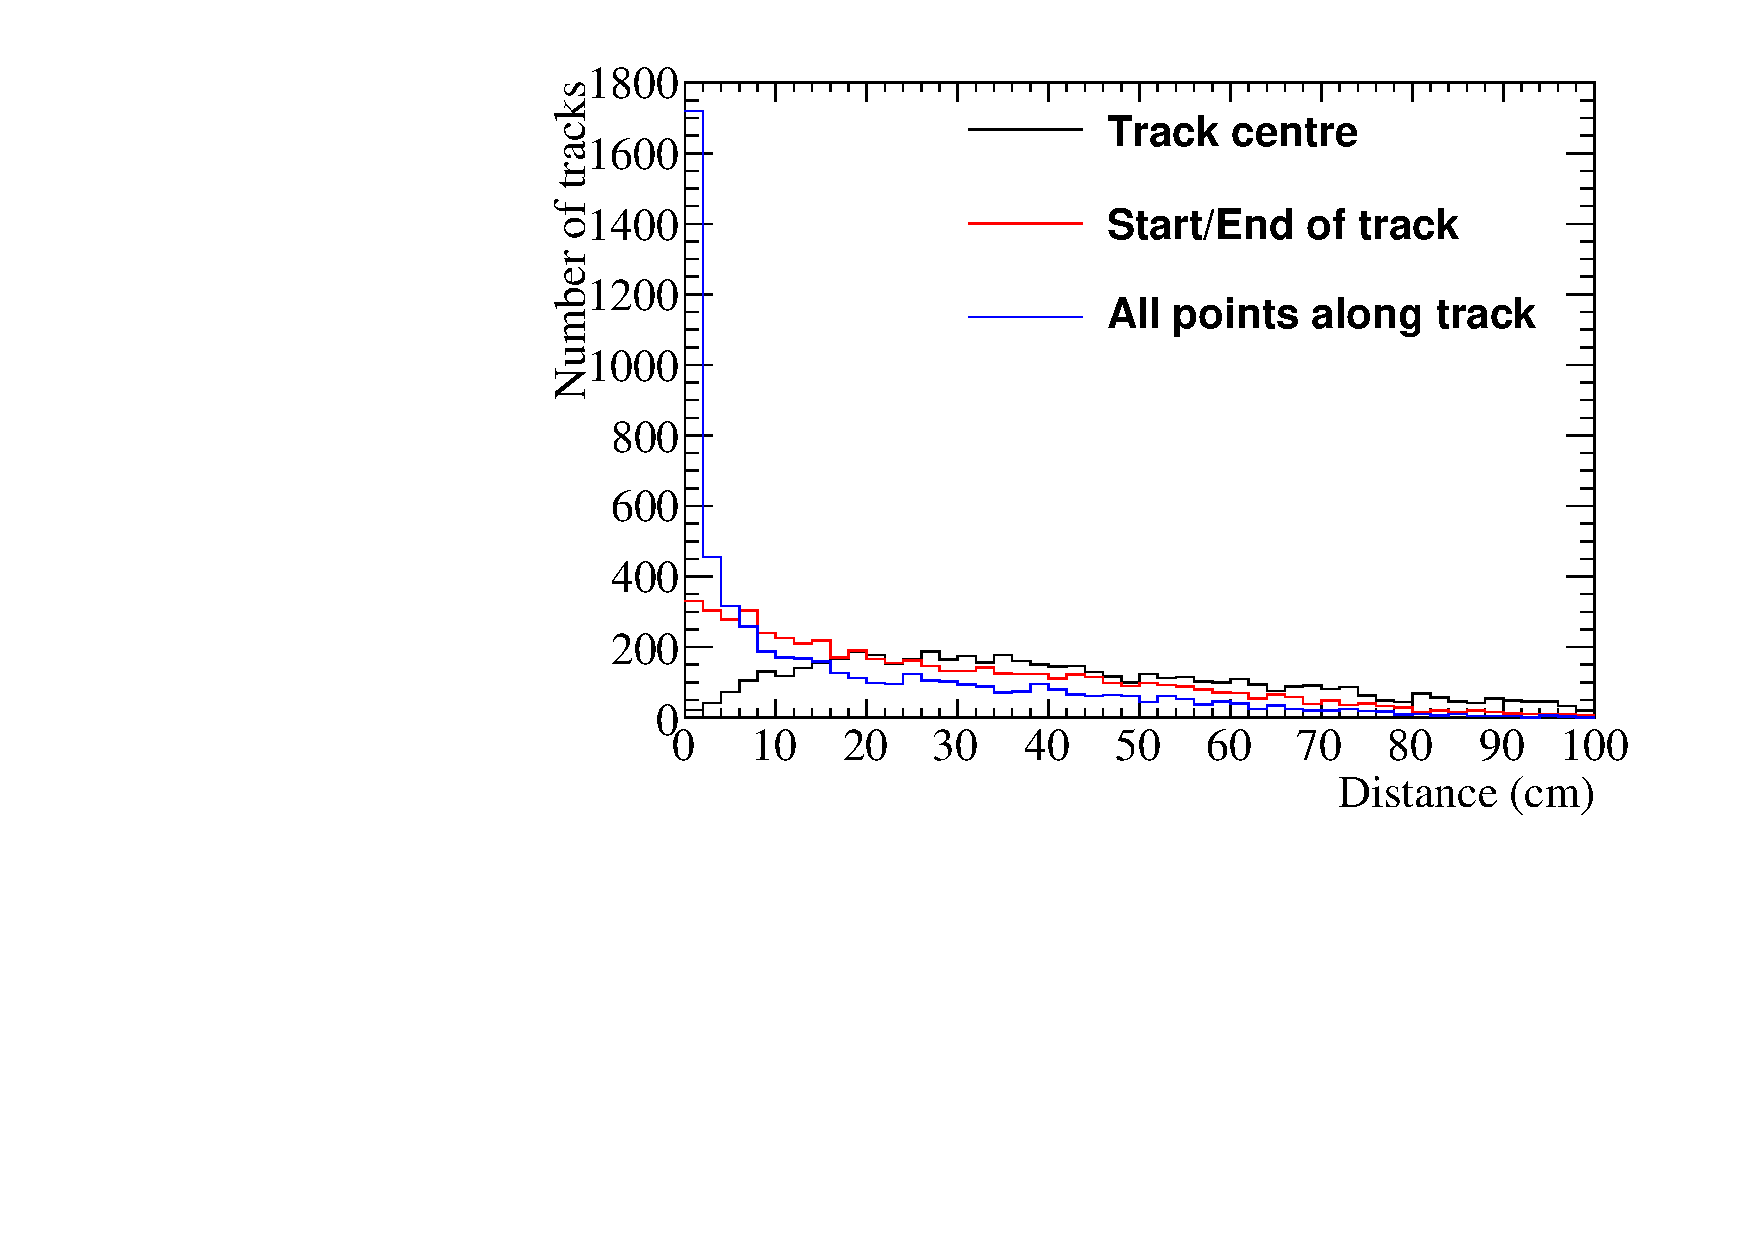
\includegraphics[width=0.5\textwidth]{DiffTrackSeps}
  \caption[Matching tracks and flashes in the 35 ton using positions in the $yz$ plane]
          {A comparison of $yz$ comparisons of reconstructed tracks and flashes in the 35 ton.}
  \label{fig:PDYZDist}
\end{figure}

Another metric by which flashes could be assigned to reconstructed tracks is by utilising the relationship between the number of measured photoelectrons and the distance from the APAs at which they were produced. When considering two flashes of scintillation light that are produced at different distances from the APAs, it would be expected that more photoelectrons would be collected from the photons produced closer to the APAs. Utilising this relationship, shown in Figure~\ref{fig:PD_PExPlot}, means that the distance from the APAs can be predicted from the number of photoelectrons which are measured. This predicted distance can then be compared to the expected $x$ position of a reconstructed track given the difference in flash time and hit times, this is shown in Figure~\ref{fig:PD_PEDiffX}. The difference in these two quantities is used as the second metric as it gives an indication of how well a flash properties match the reconstructed $x$ position of the track, with a value of 0 representing an excellent match. \\

\begin{figure}[h!]
  \centering
  \begin{subfigure}{0.45\textwidth}
    \centering
    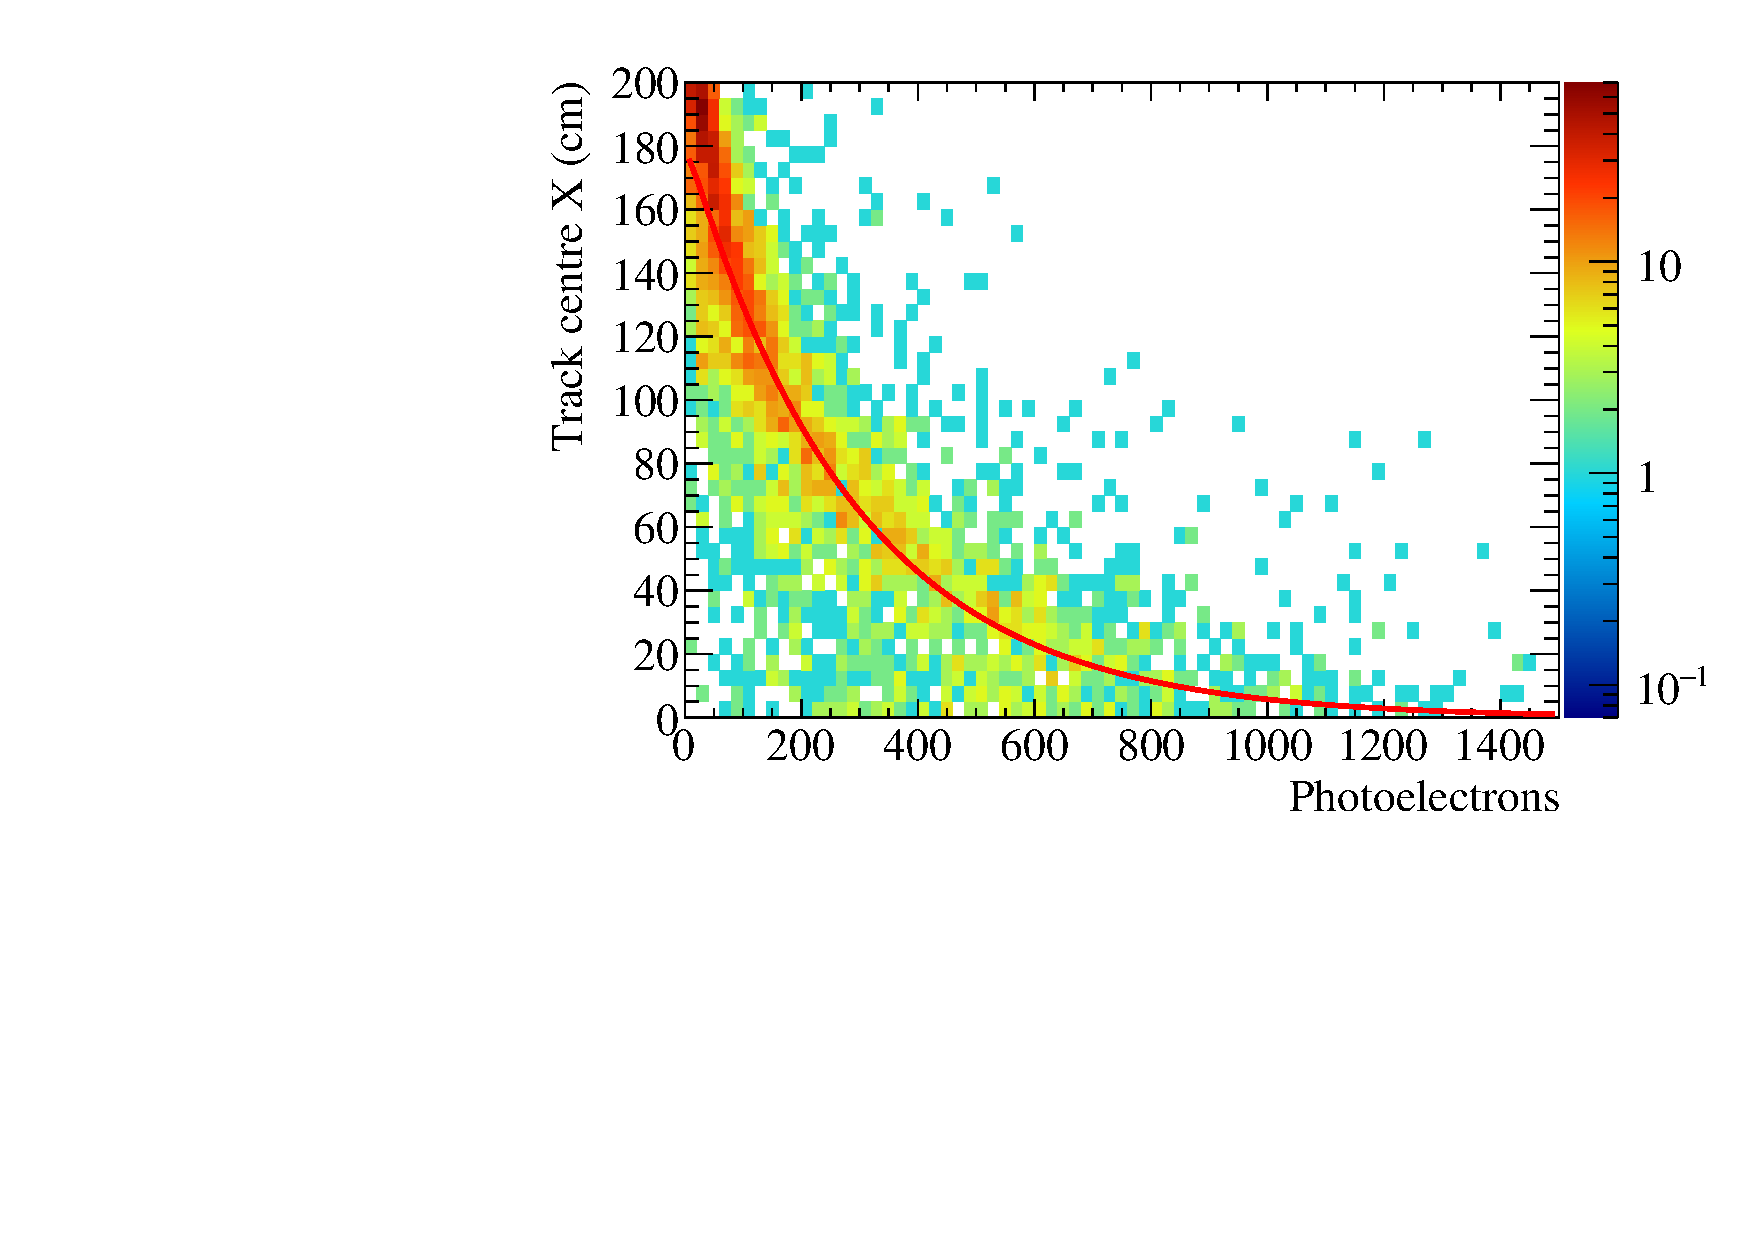
\includegraphics[width=\textwidth]{NumPE_Distance}
    \caption{How the number of photoelectrons measured changes with drift distance.}
    \label{fig:PD_PExPlot}
  \end{subfigure}
  \hspace{0.08\textwidth}
  \begin{subfigure}{0.45\textwidth}
    \centering
    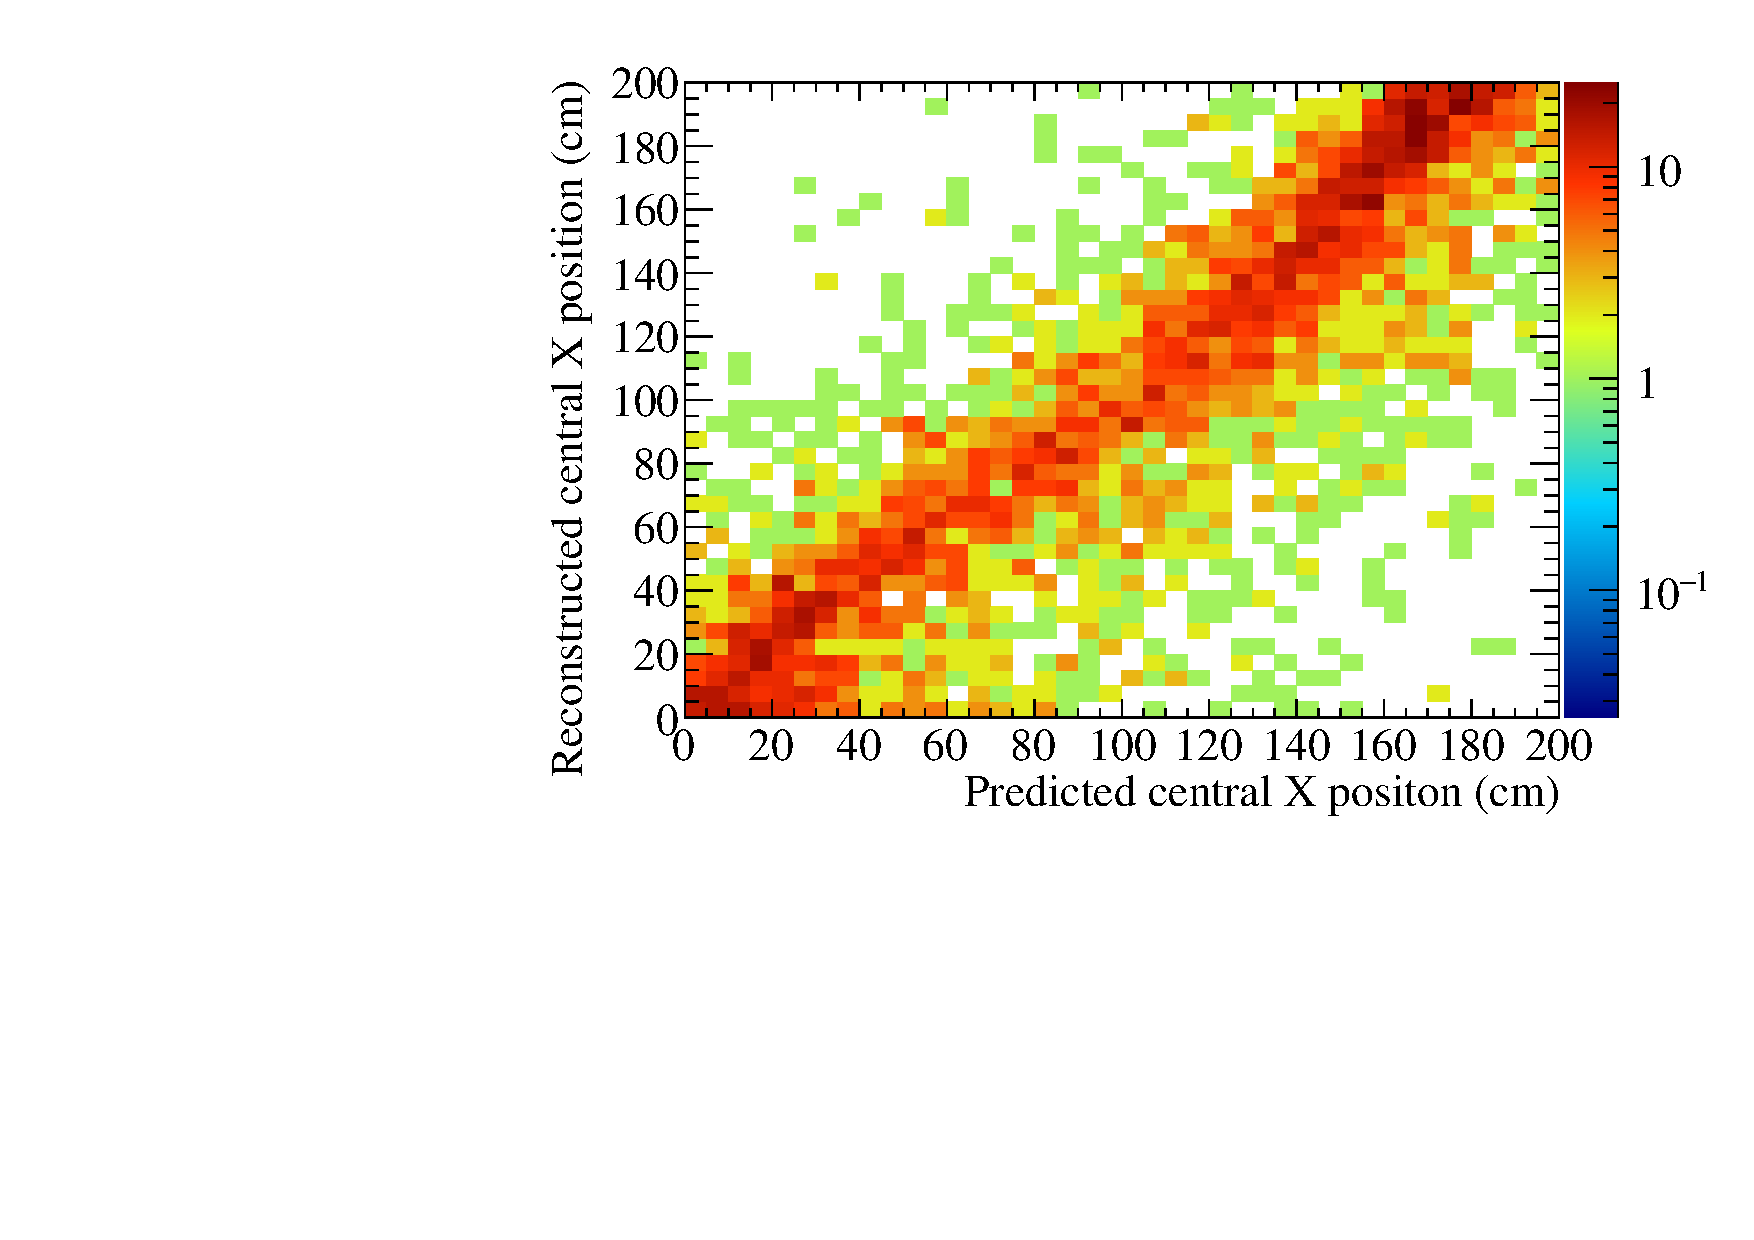
\includegraphics[width=\textwidth]{DiffFlashPredReco}
    \caption{The difference in $x$ position using the relationship in Fig~\ref{fig:PD_PExPlot} and the difference in flash and hit times.}
    \label{fig:PD_PEDiffX}
  \end{subfigure}
  \caption[Matching tracks and flashes in the 35 ton using photoelectron information]
          {How the number of reconstructed photoelectrons changes with increasing drift distance, and how this can be used to predict the interaction time of tracks. How consistent the predicted ineraction times using this method replicate the $x$ positions one would expect given the drift times they correspond to, there is one entry for every track/flash pair.}
\end{figure}

Using these metrics it is possible to attempt to assign reconstructed flashes to reconstructed tracks. Only flashes which are within one drift window of a given track are considered, as flashes outside of this time window cannot have been caused by the reconstructed track. Once flashes are assigned to tracks it is possible to determine how well the matching has performed by comparing the Monte Carlo truth interaction time with the photon detector interaction time. When doing this it is more useful to use a long (16 ms, 32,000 tick) CRY sample as then particles come at random timings as opposed to all at $T$ = 0 as with the Anti-Muon sampe initially considered. This comparison is shown in Figure~\ref{fig:PD_MCPDDiff}, where there is a clear peak at a time difference of 0 $ms$ in the Monte Carlo truth and photon detector interaction times. When zooming in on this peak it can be seen that there is a systematic offset of 0.6 $\mu$s, this is due to an electronics offset applied in the simulation to the photon detector system. \\

\begin{figure}[h!]
  \centering
  \begin{subfigure}{0.45\textwidth}
    \centering
    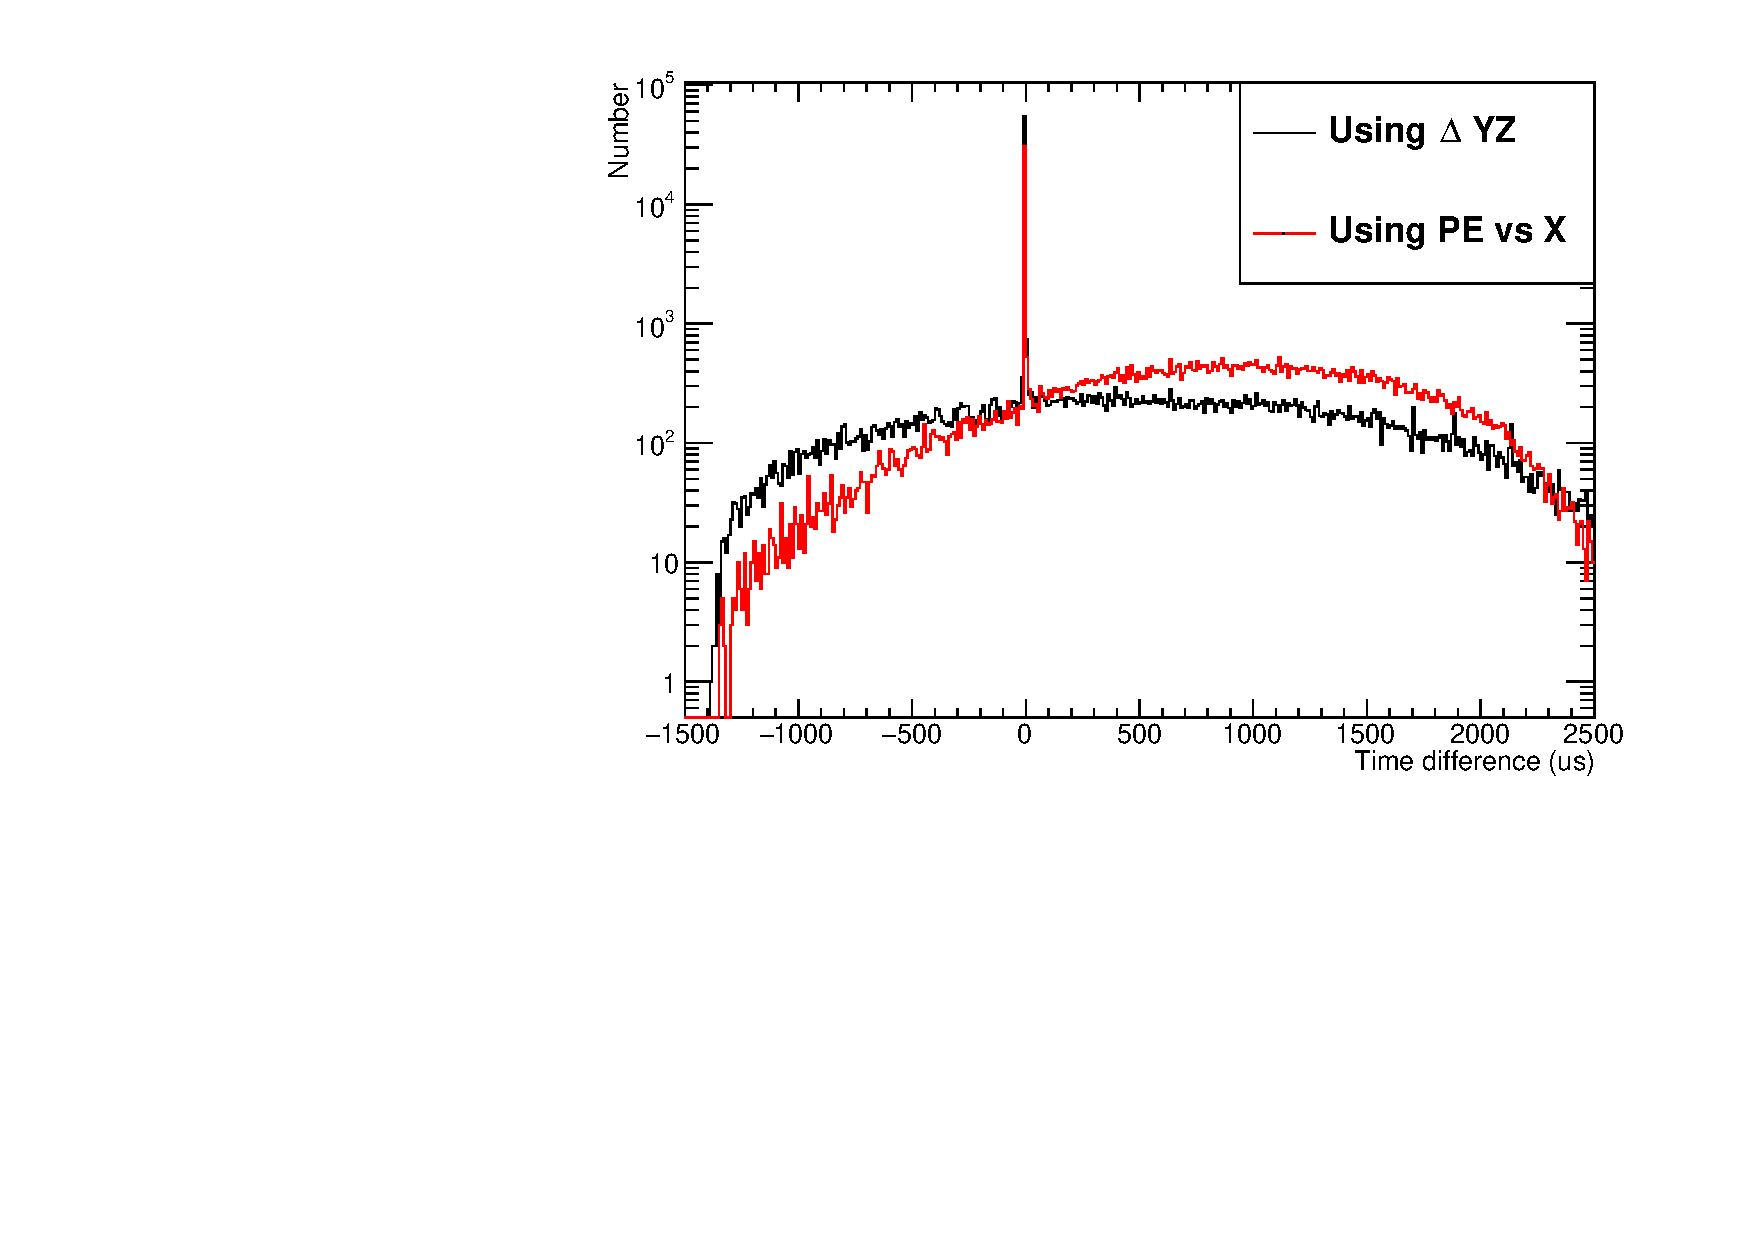
\includegraphics[width=\textwidth]{Pred_Reco_T_Full}
    \caption{The difference in interaction times.}
  \end{subfigure}
  \hspace{0.08\textwidth}
  \begin{subfigure}{0.45\textwidth}
    \centering
    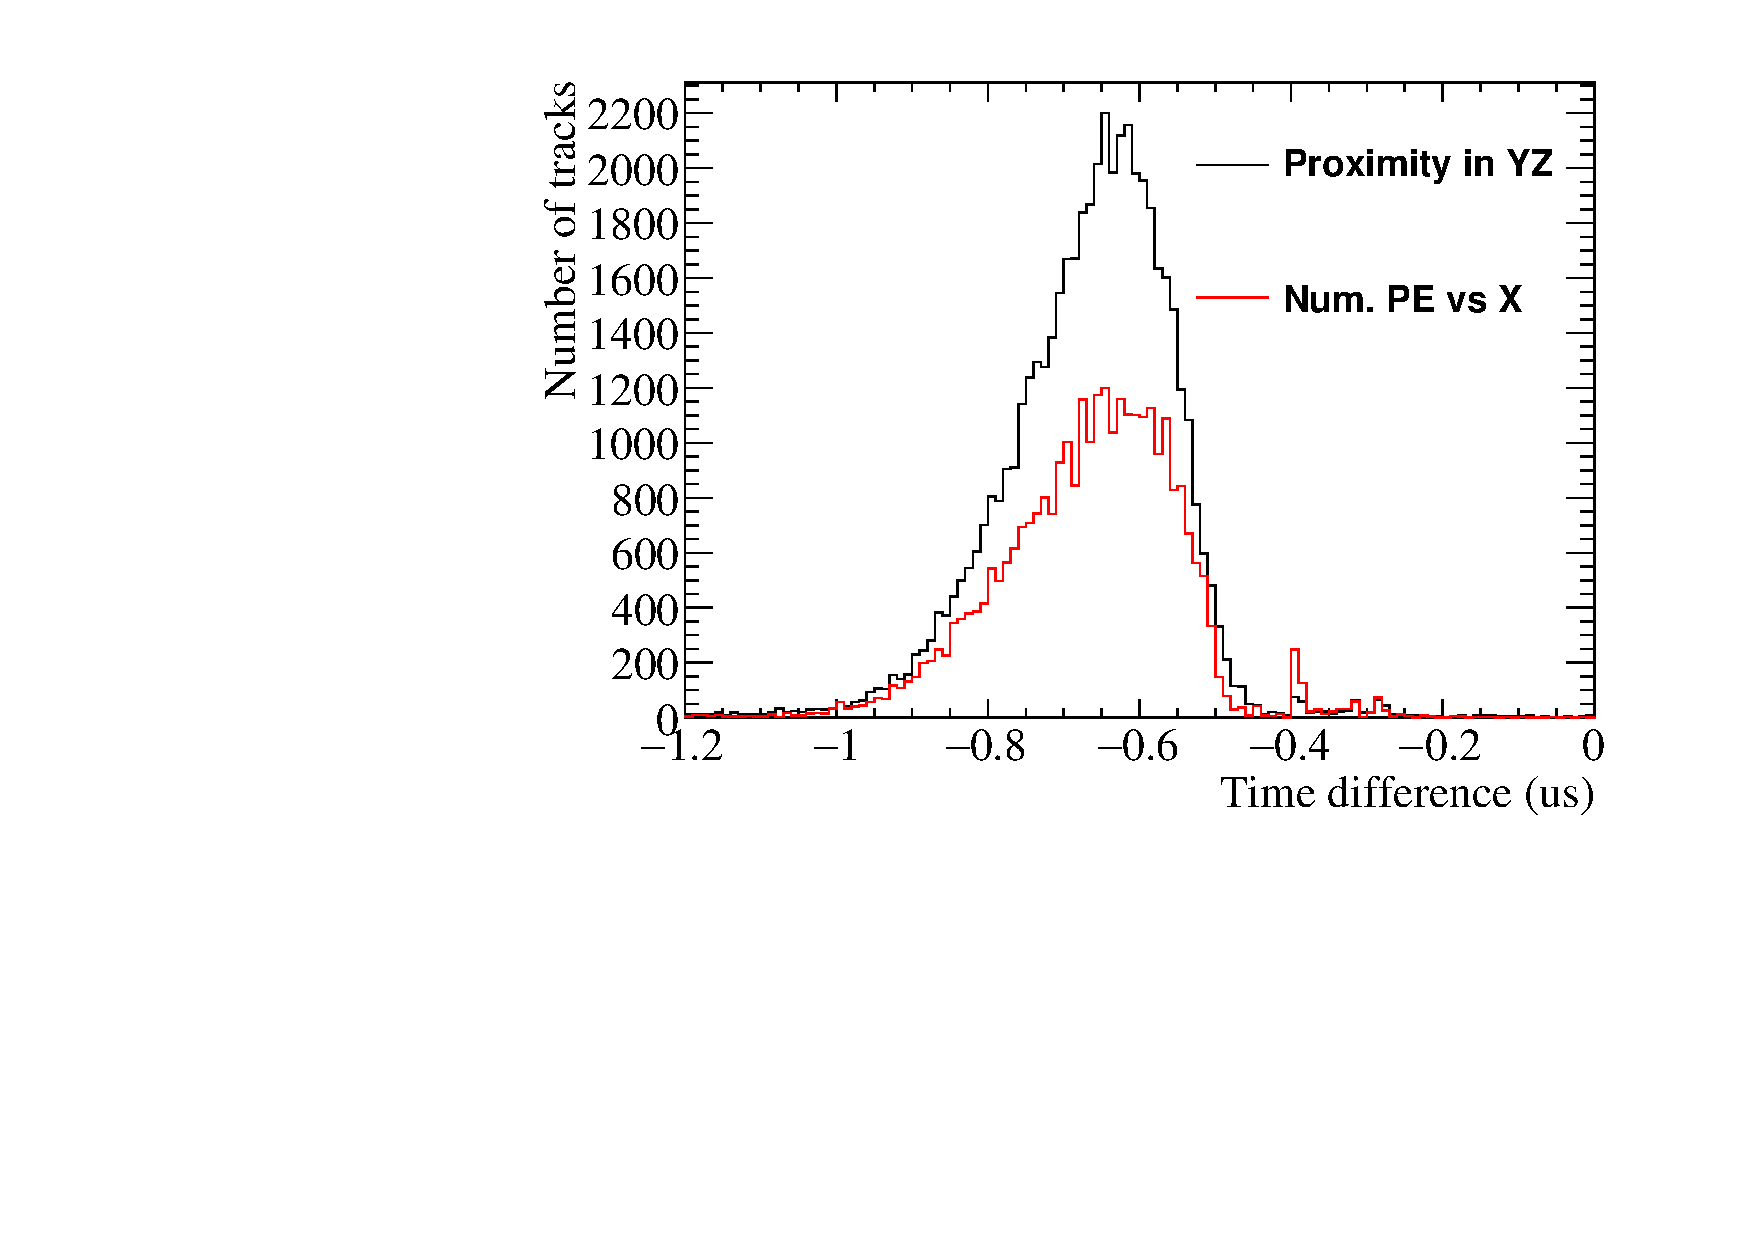
\includegraphics[width=\textwidth]{Pred_Reco_T_Zoom}
    \caption{Zoomed in at low time differences.}
  \end{subfigure}
  \caption[The difference in Monte Carlo interaction times and the predicted interaction times using the photon detectors]
          {The difference in Monte Carlo interaction times and the predicted interaction times using the photon detectors.}
          \label{fig:PD_MCPDDiff}
\end{figure}

From Figure~\ref{fig:PD_MCPDDiff} it can clearly be seen that the metric using the proximity of the flash centre to the track trajectory yields the best matches. This is likely caused by the large spread in the number of photoelectrons collected at fixed drift distances, as shown by Figure~\ref{fig:PD_PExPlot}. The two metrics can be combined to give a prediction for the interaction time, though given the increased sensitivity from the proximity metric this should be given greater weighting. In physics data the metric using the number of collected photoelectrons is particularly sensitive to the absolute light level in the detector as a high residual light level would reduce the proportional change in the number of photonelectrons collected for increasing drift distances. This metric also relies a sample of tracks with known $x$ positions upon which it can be calibrated which may be difficult to obtain. \\



%********************************** % Second Section  *************************************
\section{Calibrating calorimetric constants} \label{sec:MCCalib} %Section - X.2
Having the correct calorimetric responses is vital when trying to calculate $\frac{dE}{dx}$ as the measured change in charge has to be correctly converted to the change in energy. The parameters which need to be tuned in order to ensure that this is doen correctly are the $Recomb_A$ and $Recomb_B$ of Equations~\ref{eq:ModBox},~\ref{eq:ModBox_B},~\ref{eq:Birks_A} and~\ref{Birks_B} respectively. These parameters have to be tuned in such a way as to make a known particle energy deposition have the correct $\frac{dE}{dx}$, the easiest deposition to tune against is the Minimally Ionising Particle (MIP) peak which in LAr should have a value of 1.8 MeV cm$^{-3}$. To do this the sample of 10,000 Anti-Muons made to calibrate the photon detector track/flash assignment will be used as many of these particles will be MIPs. \\

To select the MIPs in the sample only tracks caused by through-going muons are used. The $\frac{dE}{dx}$ value for all hits in all tracks is then calculated, with the different planes separated out as each one will have its own normalisation factor. A Guassian distribution is then fitted around the peaks for each of the planes to discern the Most Probable Value (MPV) of $\frac{dE}{dx}$ for that plane. If the MPVs are not equal to 1.8 MeV cm$^{-3}$ then the normalisation factors are scaled through a process of trial and error until the correct MPVs are measured. An example of the tuning being applied is shown in Figure~\ref{fig:CaloTune}. Tuning of the calorimetric constants is requried whenever the electronics gains or signal shaping functions are changed.

\begin{figure}[h!]
  \centering
  \begin{subfigure}{0.45\textwidth}
    \centering
    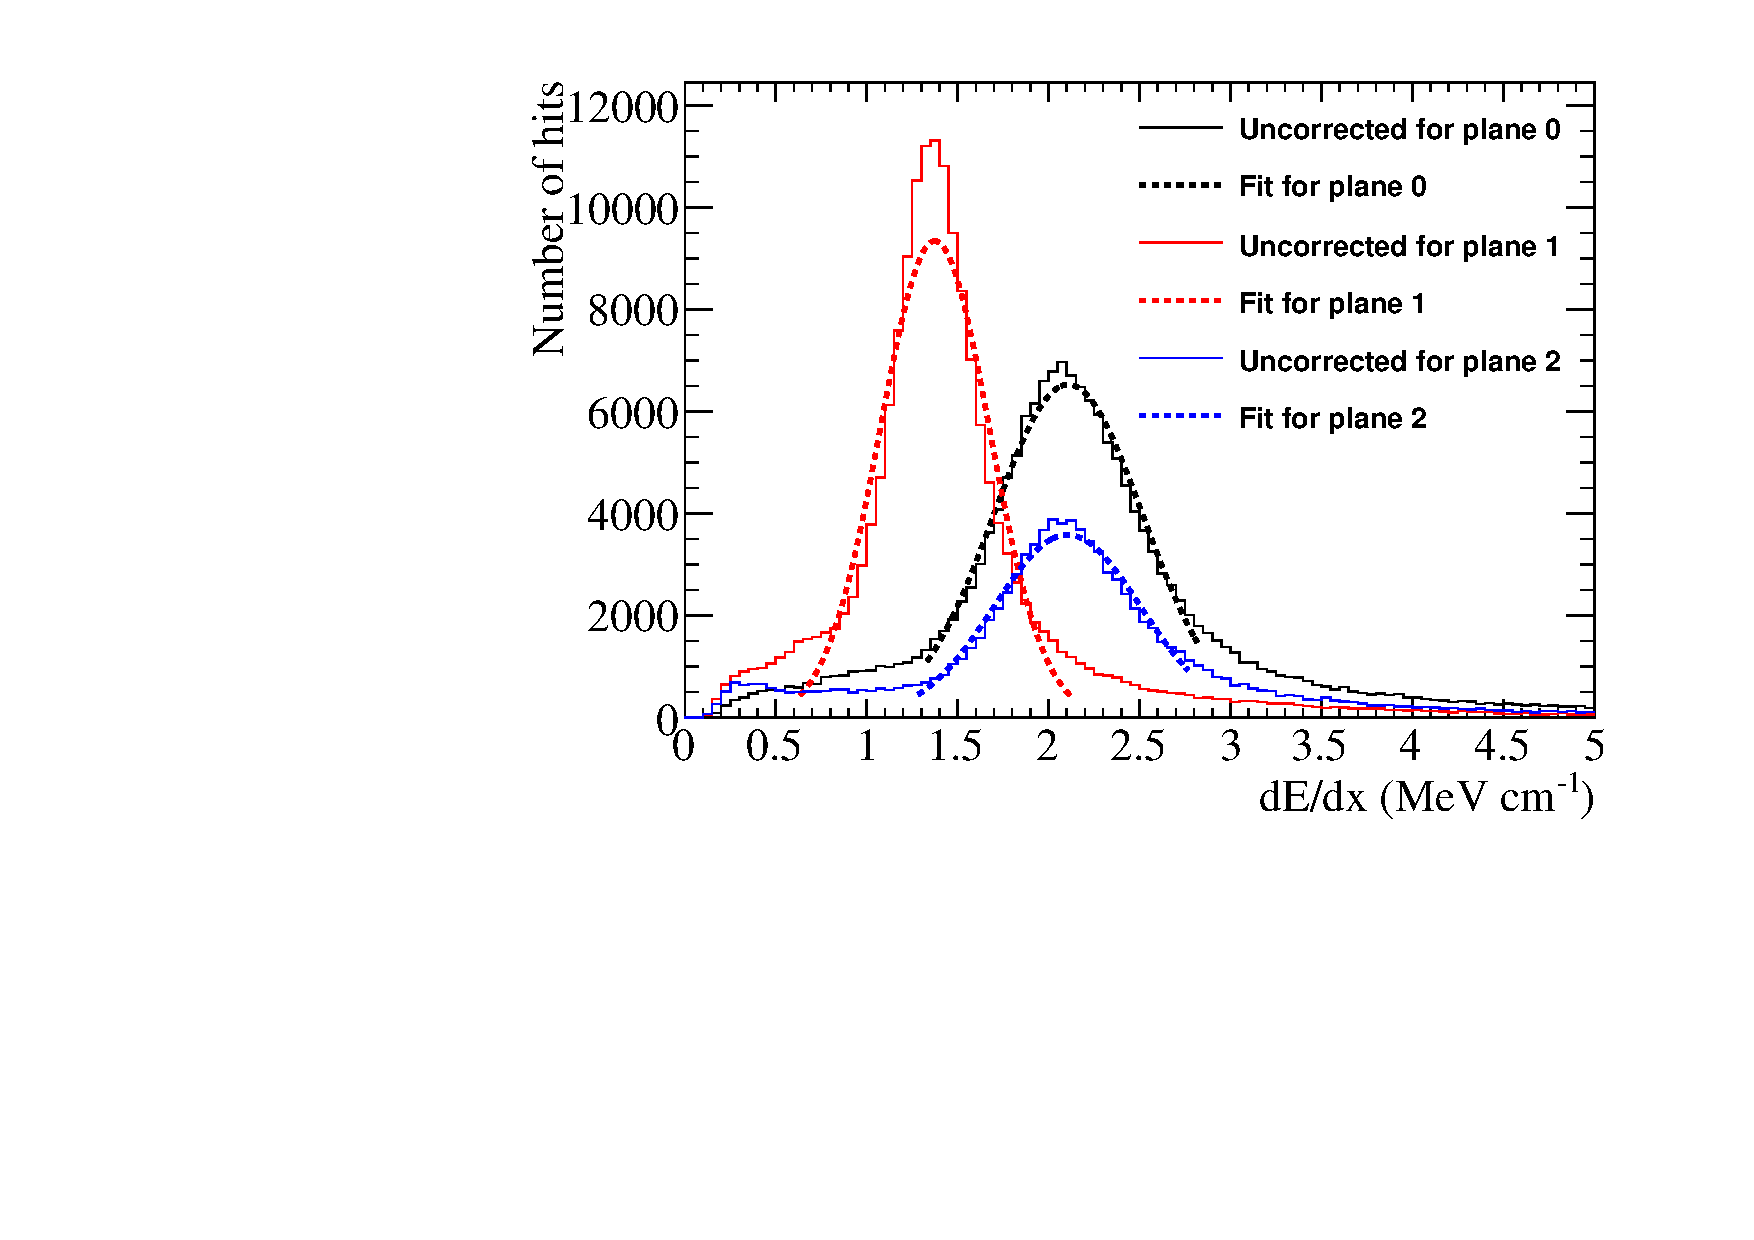
\includegraphics[width=\textwidth]{UnCorrectedCanvas}
    \caption{Before a normalisation correction is applied.}
    \label{fig:CaloTune_Before}
  \end{subfigure}
  \hspace{0.08\textwidth}
  \begin{subfigure}{0.45\textwidth}
    \centering
    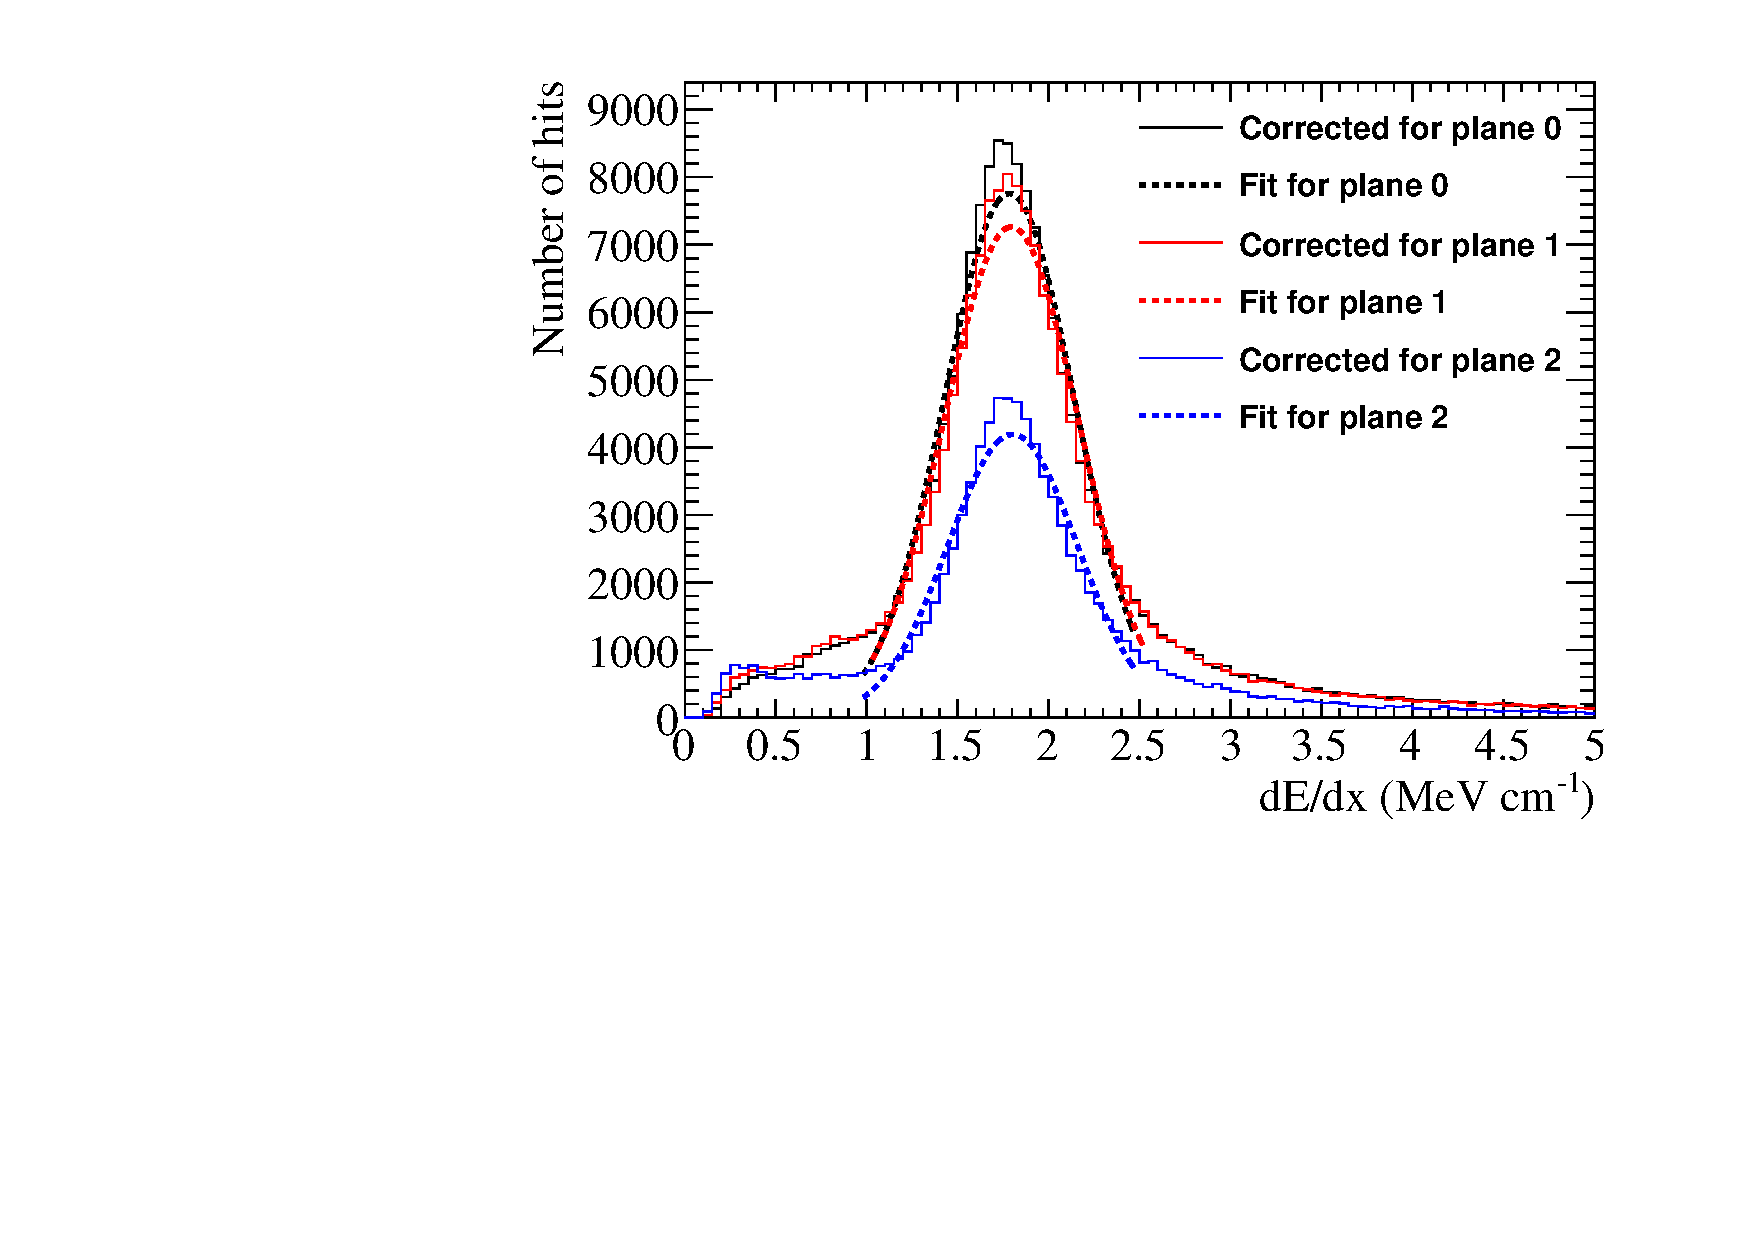
\includegraphics[width=\textwidth]{CorrectedCanvas}
    \caption{After a normalisation correction is applied.}
    \label{fig:CaloTune_After}
  \end{subfigure}
  \caption[The tuning of the calorimetric constants in the 35 ton]
          {How the $\frac{dE}{dx}$ MPVs change for each plane when a change is made to the electronics gains in the 35 ton. Figure~\ref{fig:CaloTune_Before} shows the MPVs after the change using the previous constants, whilst Figure~\ref{fig:CaloTune_After} shows the MPVs after a retuning of the constants.}
          \label{fig:CaloTune}
\end{figure}
        
%********************************** % Third Section  *************************************
\section{Discerning reconstruction efficiencies} \label{sec:SimRecoEffic} %Section - X.3
Knowledge of the strengths and weaknesses of different tracking algorithms is vital when using them for physics analyses, to this end it is useful to develop a metric by which they can be compared. In order to do this a series of conditions have to be applied to the reconstructed tracks from a large set of simulated particles which are reconstructed using different tracking algorithms. It is interesting to observe what the effect of event complexity has on the reconstruction algorithms and so efficiencies will be calculated for both the Anti-Muon and CRY samples used in Section~\ref{sec:SimInteractionTimes}. \\

The critera upon which to determine whether a particle is well reconstructed has to be carefully chosen as every definition will have limitations. For example, consider a particle that travels 100 cm in the active volume of the detector but is reconstructed as 2 separate tracks (tracks 1 and 2), with lengths 77 cm and 23 cm respectively. Firstly, should these tracks should be merged, or left separate? If the reconstruction algorithms have found them to be separate tracks then it would be difficult to ascertain that they are from the sample particle in real data, and so in considerations here they are not merged. One metric of efficiency would be to consider a track well reconstructed if it has a length between 75$\%$ and 125$\%$ of the Monte Carlo truth length that the particle traversed in the detector, in which case track 1 would be considered well reconstructed. Another metric however would be to consider a track well reconstructed if the Monte Carlo truth distance the particle traversed in the detector is between 75$\%$ and 125$\%$ of the reconstructed length, in which case neither track would be considered well matched. Both metrics have used exactly the same tracks and a seemingly identical method of evaluating whether a track is well reconstructed or not, but have got the opposite results. As such it is wrong to say which consideration gives the correct result, but instead the result of each should be considered equally. In discussions here the former definition of efficency will be used, such that a track is considered well reconstructed if:
\begin{itemize}
\item Reconstructed track length is more than or equal to 75$\%$ of the Monte Carlo track length.
\item Reconstructed track length is less than or equal to 125$\%$ of the Monte Carlo track length.
\item Only one reconstructed track can be matched per Monte Carlo particle.
\end{itemize}

When calculating efficiencies it is important to consider much more than just the ratio of reconstructed to true track length. To this end efficiencies with regards to many aspects of the tracks are calculated:
\begin{itemize}
\item Track length
\item Energy deposited in the active volume of the detector
\item The angle $\theta$ of the track
\item The angle $\phi$ of the track
\end{itemize}
In all efficiency plots the Monte Carlo truth quantity, not the reconstructed quantity is shown so as to reflect how the variations of these quantities affect the reconstruction efficiencies. It is also useful to observe the effect on reconstruction of failed disambiguation and incorrect interaction time determination. To show this two forms of reconstruction are ran on the particles, one no Monte Carlo information is used and another where the disambiguation and interaction time are cheated. Cheated disambiguation means using the Monte Carlo truth information of the energy despoition to correctly assign which wire segment the energy was deposited on. \\

The calculation of reconstruction efficiencies also serves as an effective method upon which reconstruction algorithms can be further developed as it identifies aspects which do not work as expected. For example when the efficiencies for the CRY sample were initially calculated they were significantly lower than for the Anti-Muon sample, but only when disambiguation was not cheated. It transpired that this was because the disambiguation was only selecting the largest collection of hits on each plane for each TPC. This is not a problem when only 1 particle is simulated and will reduce the number of noise hits but in a CRY sample of 16 ms there will almost certainly be multiple particles in each TPC. Removing the hits from all but one of these multiple particles will cause them to have no reconstructed track, and thus cause the efficiency to drop significantly. Upon making the dismabiguation algorithm no longer have this restriction the reconstruction efficiencies of the Anti-Muon and CRY samples were observed to become much more similar. \\

The reconstruction efficiencies given the current state of the most commonly used reconstruction algorithms are shown in Figures~\ref{fig:SimEffic_Length},~\ref{fig:SimEffic_EnDepos},~\ref{fig:SimEffic_Theta},~\ref{fig:SimEffic_Phi} and~\ref{fig:SimEffic_ThetaPhi}. Efficiences are shown for both the Anti-Muon and CRY samples, where it can be seen that the efficiency tends to be lower for the CRY sample. It is thought that this is due to the more complex event structure, as particles will have large interaction times and particles which have similar interaction times may cross causing reconstruction errors. The reconstruction efficiencies for the CRY sample are more realistic as events will rarely be isolated in the detector due to the large flux of cosmic particles on the Earth's surface. \\

\begin{figure}[h!]
  \centering
  \begin{subfigure}{0.45\textwidth}
    \centering
    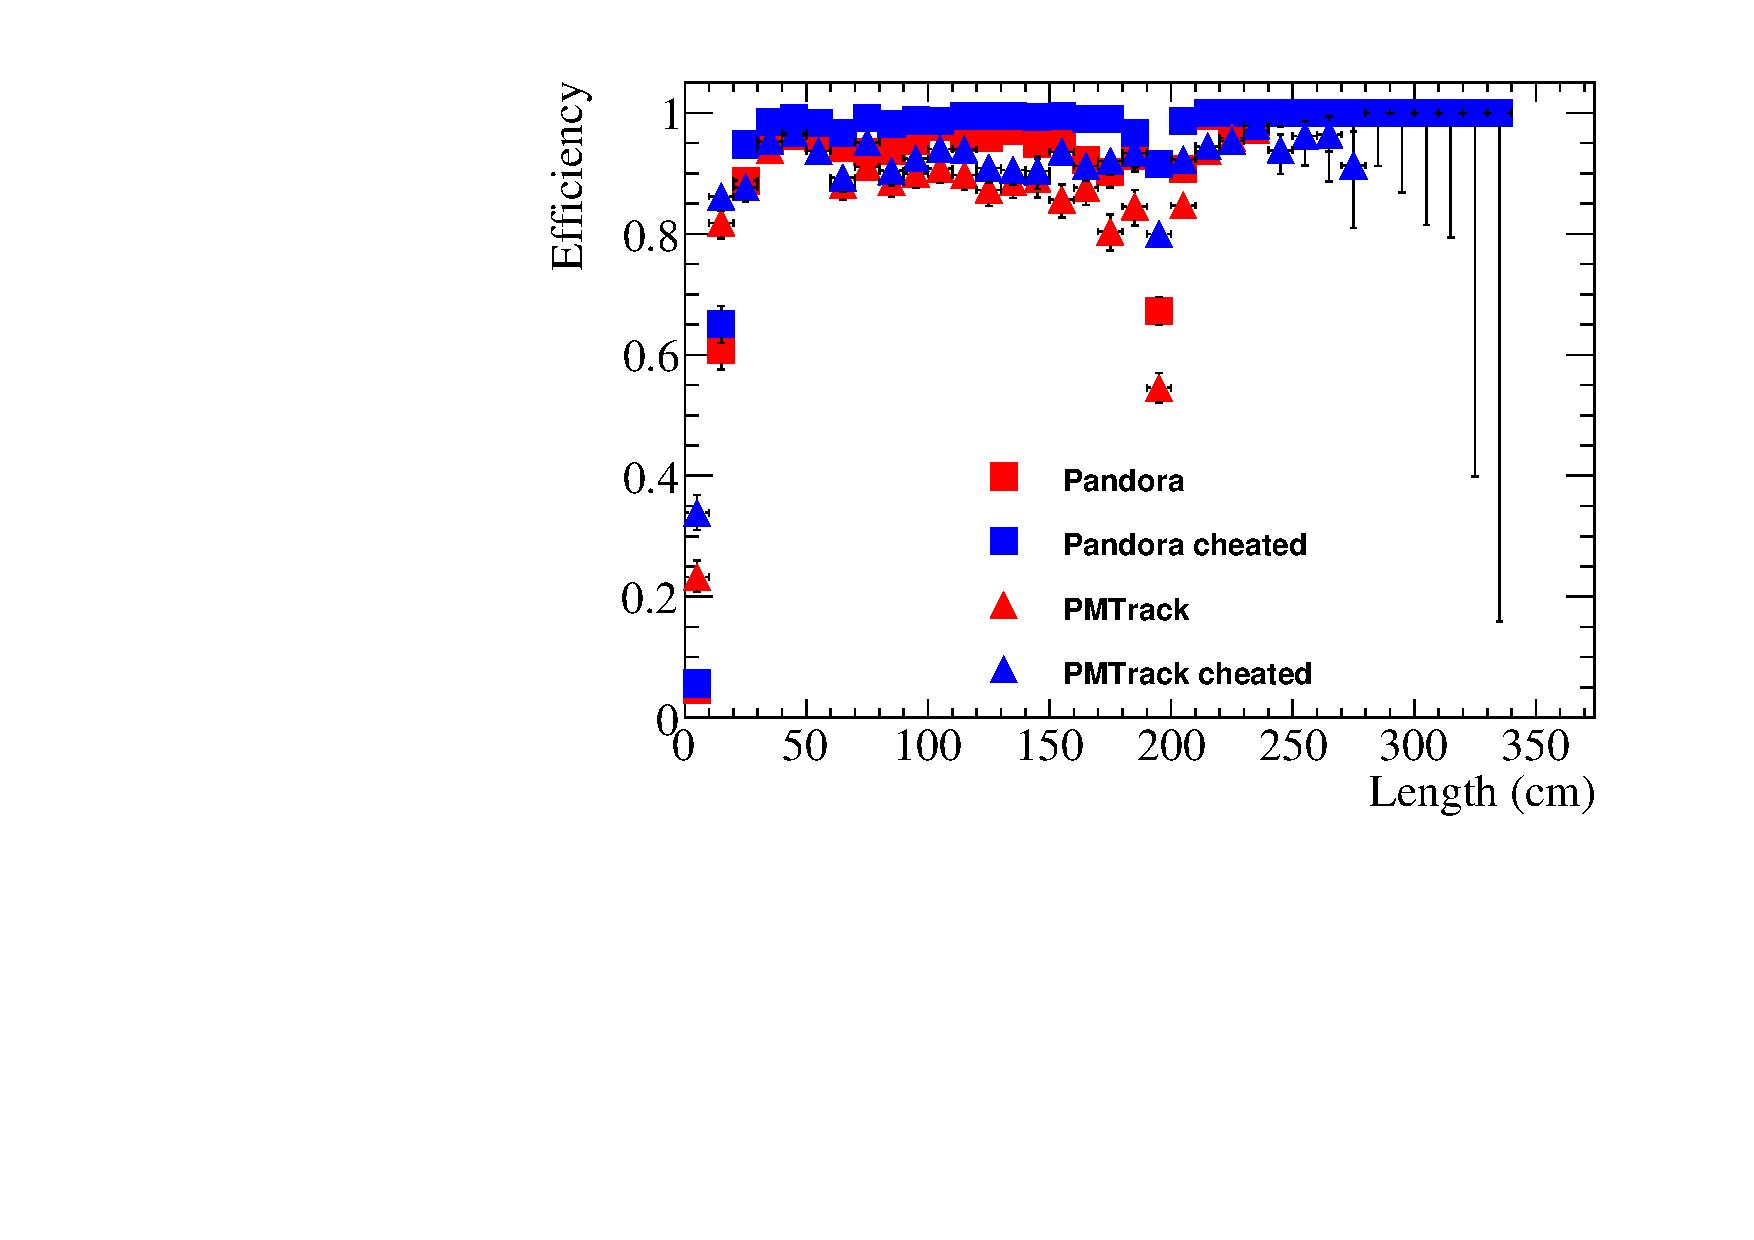
\includegraphics[width=\textwidth]{Effic_AntiMuon_500V_All_Length}
    \caption{Reconstruction efficiencies for an Anti-Muon sample.}
    \label{fig:SimEffic_Length_AMu}
  \end{subfigure}
  \hspace{0.08\textwidth}
  \begin{subfigure}{0.45\textwidth}
    \centering
    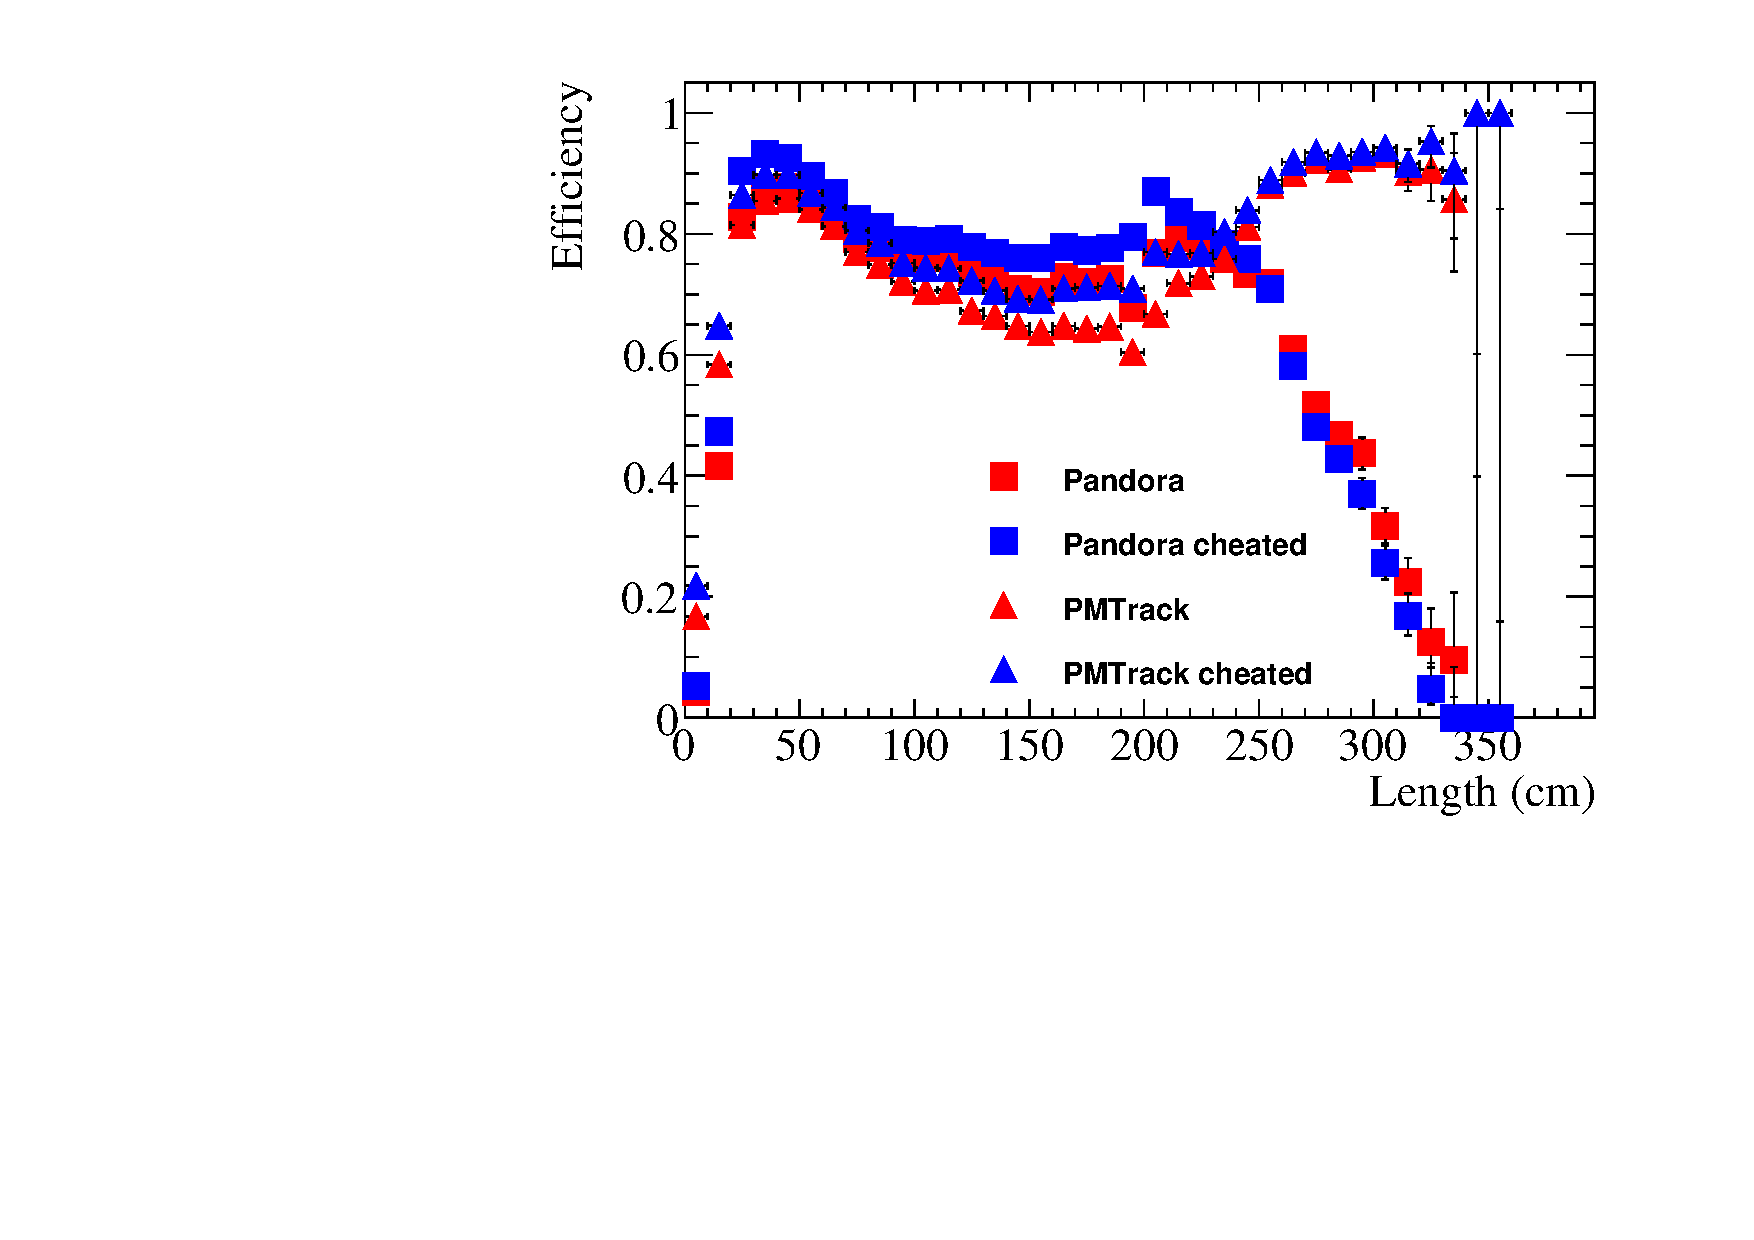
\includegraphics[width=\textwidth]{Effic_Cosmics_500V_All_Length}
    \caption{Reconstruction efficiencies for a CRY sample.}
    \label{fig:SimEffic_Length_CRY}
  \end{subfigure}
  \caption[The reconstruction efficiencies for simulated events as a function of Monte Carlo truth track length.]
          {The reconstruction efficiencies for simulated events as a function of Monte Carlo truth track length. The efficiencies are shown for non-cheated reconstruction (square blocks) and cheated reconstruction (triangle blocks) for both PMTrack (black) and Pandora (blue).}
          \label{fig:SimEffic_Length}
\end{figure}

\begin{figure}[h!]
  \centering
  \begin{subfigure}{0.45\textwidth}
    \centering
    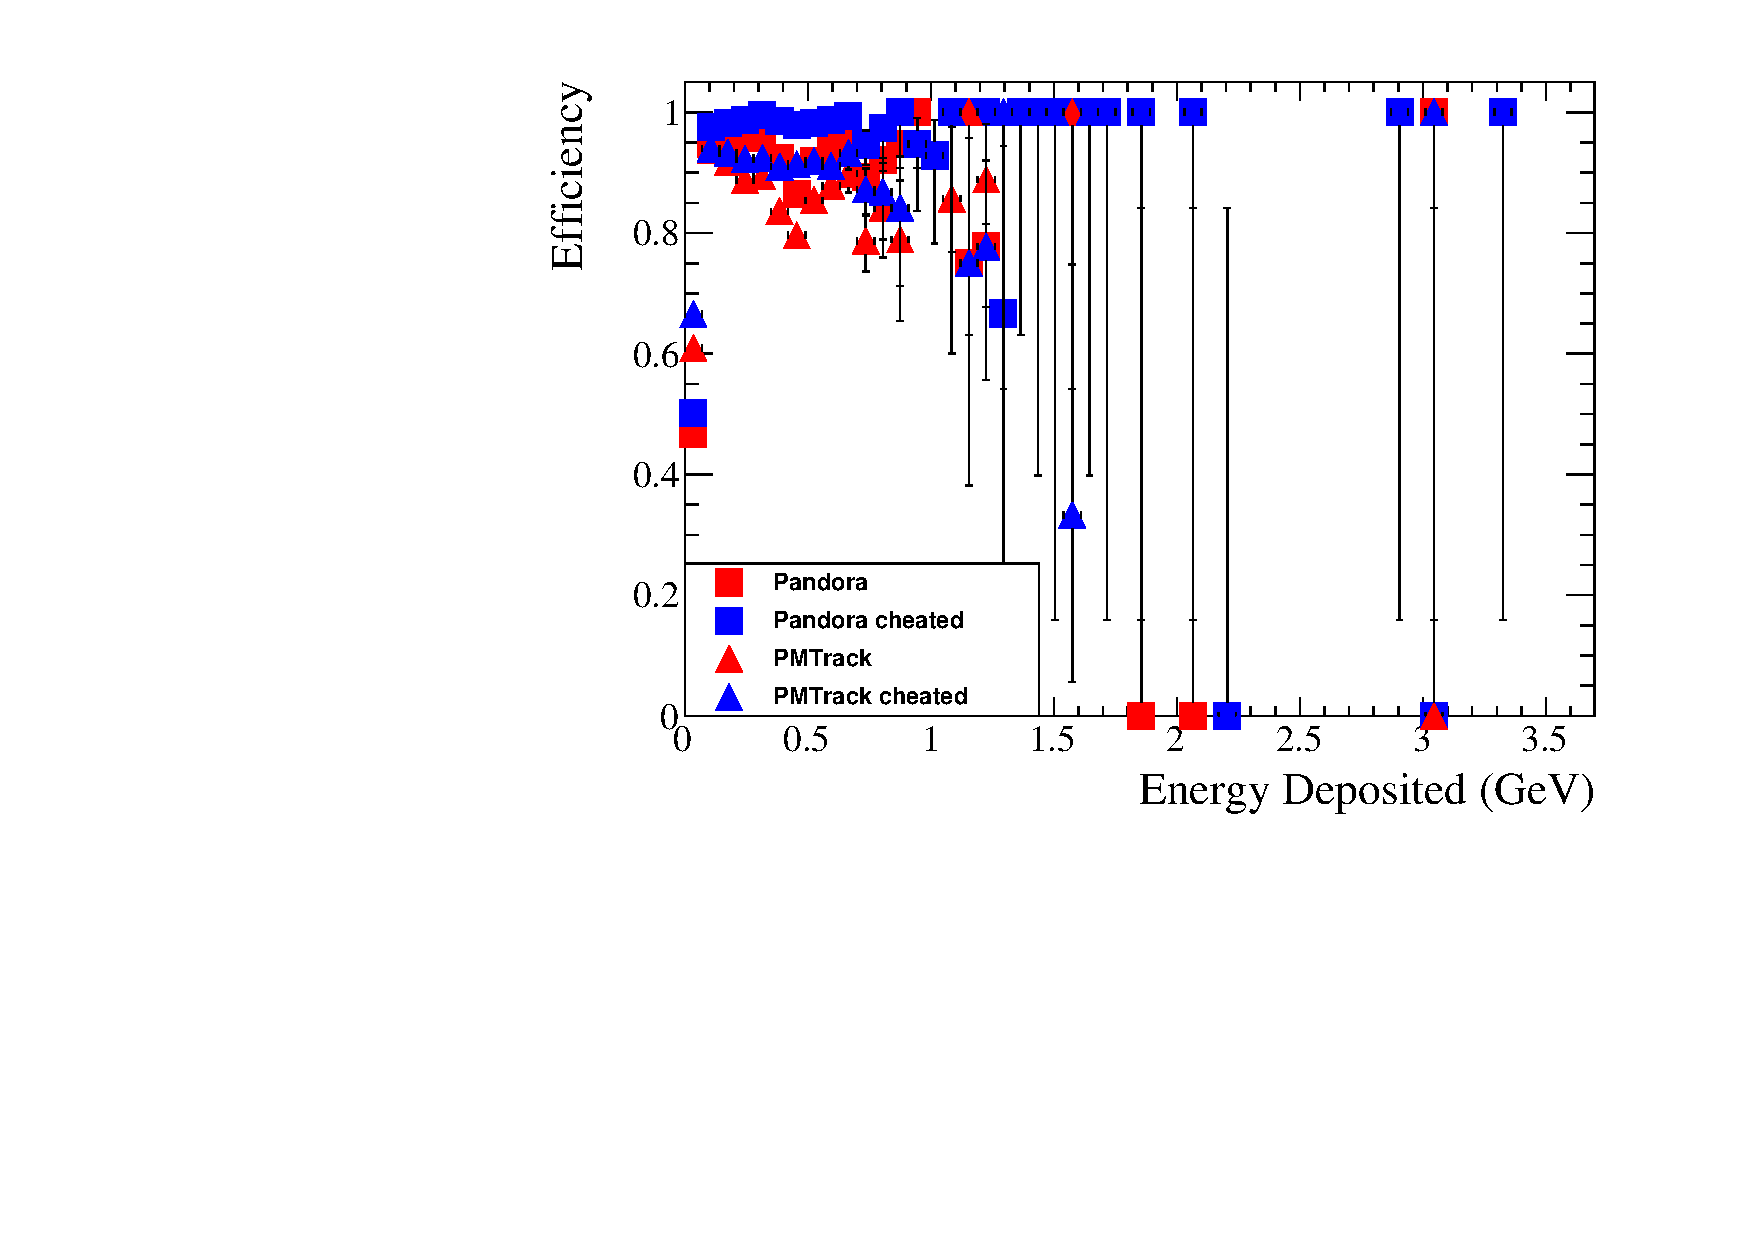
\includegraphics[width=\textwidth]{Effic_AntiMuon_500V_All_EnDepos}
    \caption{Reconstruction efficiencies for an Anti-Muon sample.}
    \label{fig:SimEffic_EnDepos_AMu}
  \end{subfigure}
  \hspace{0.08\textwidth}
  \begin{subfigure}{0.45\textwidth}
    \centering
    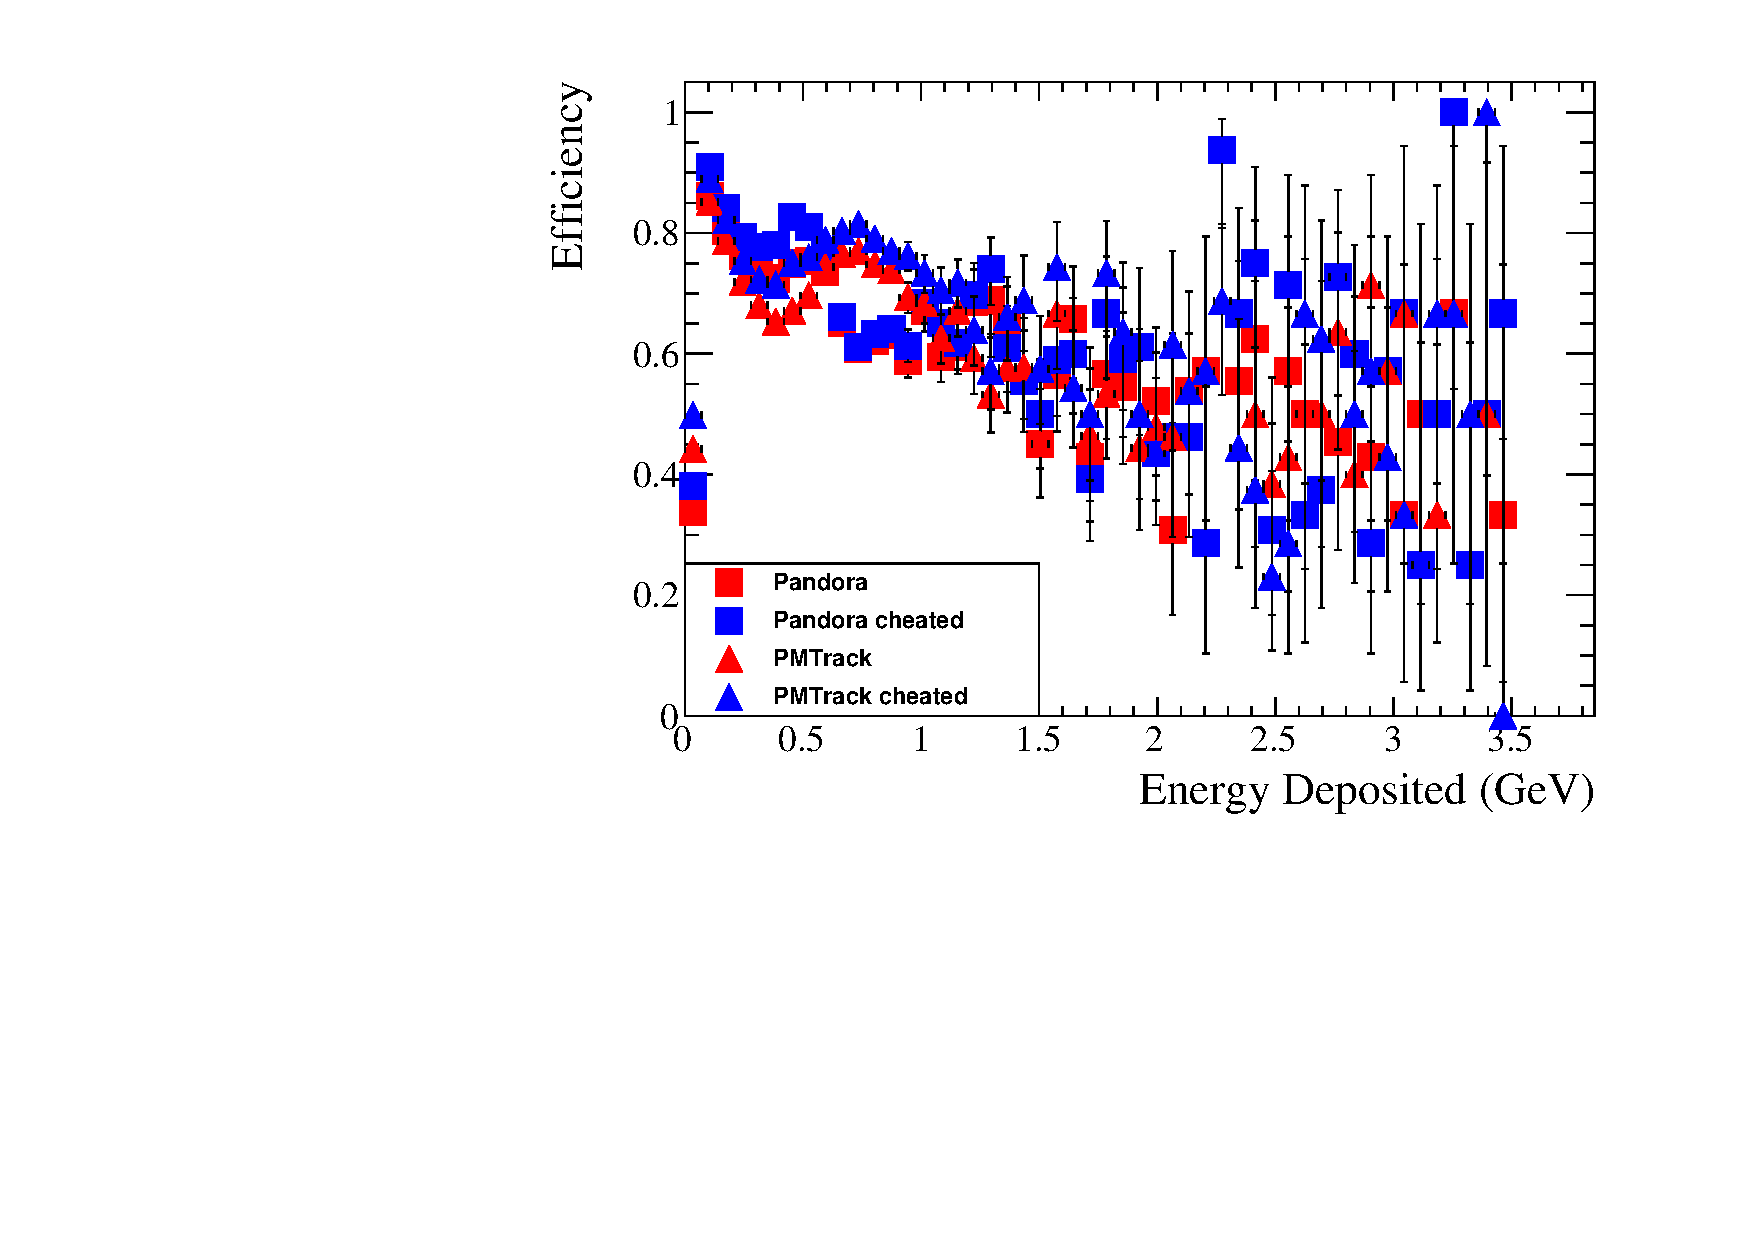
\includegraphics[width=\textwidth]{Effic_Cosmics_500V_All_EnDepos}
    \caption{Reconstruction efficiencies for a CRY sample.}
    \label{fig:SimEffic_EnDepos_CRY}
  \end{subfigure}
  \caption[The reconstruction efficiencies for simulated events as a function of Monte Carlo truth deposited energy.]
          {The reconstruction efficiencies for simulated events as a function of Monte Carlo truth deposited energy. The efficiencies are shown for non-cheated reconstruction (square blocks) and cheated reconstruction (triangle blocks) for both PMTrack (black) and Pandora (blue).}
          \label{fig:SimEffic_EnDepos}
\end{figure}

\begin{figure}[h!]
  \centering
  \begin{subfigure}{0.45\textwidth}
    \centering
    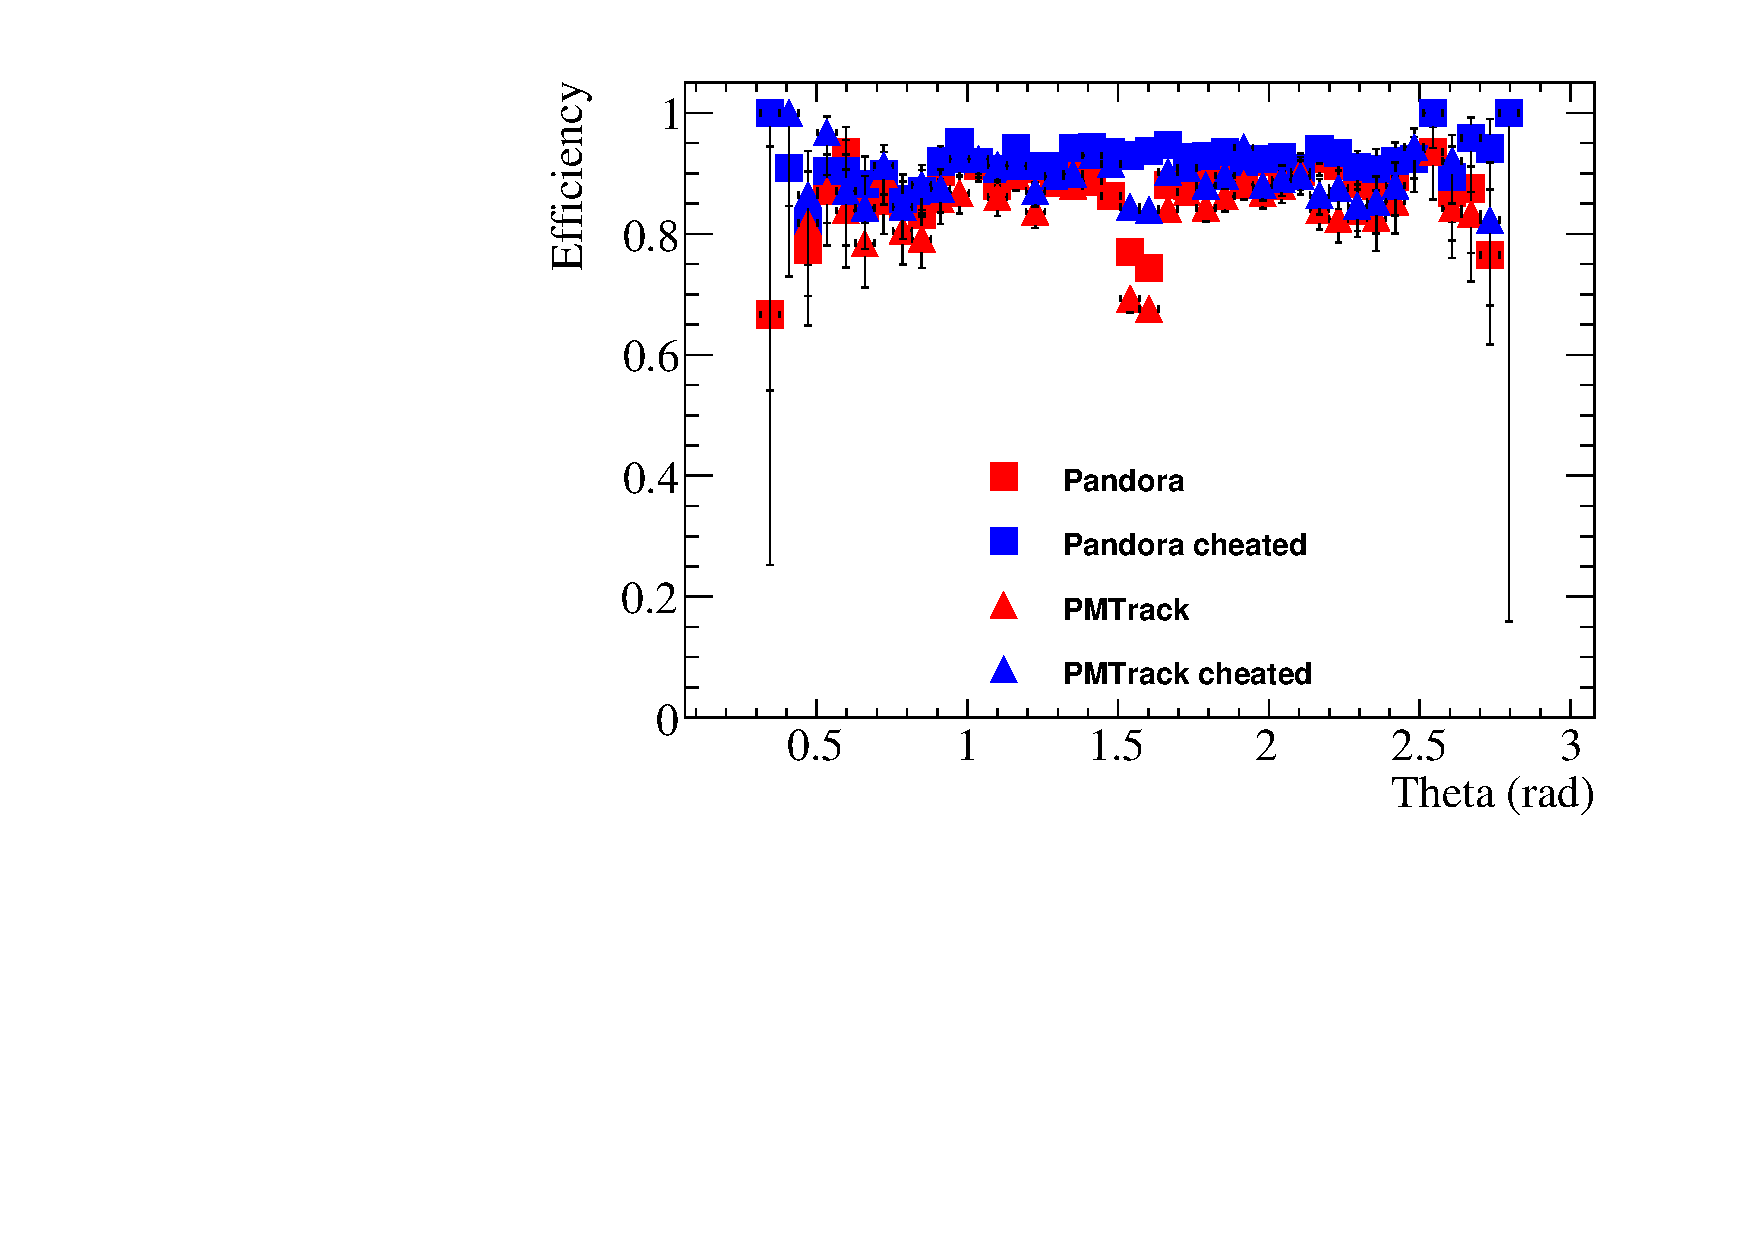
\includegraphics[width=\textwidth]{Effic_AntiMuon_500V_All_Theta}
    \caption{Reconstruction efficiencies for an Anti-Muon sample.}
    \label{fig:SimEffic_Theta_AMu}
  \end{subfigure}
  \hspace{0.08\textwidth}
  \begin{subfigure}{0.45\textwidth}
    \centering
    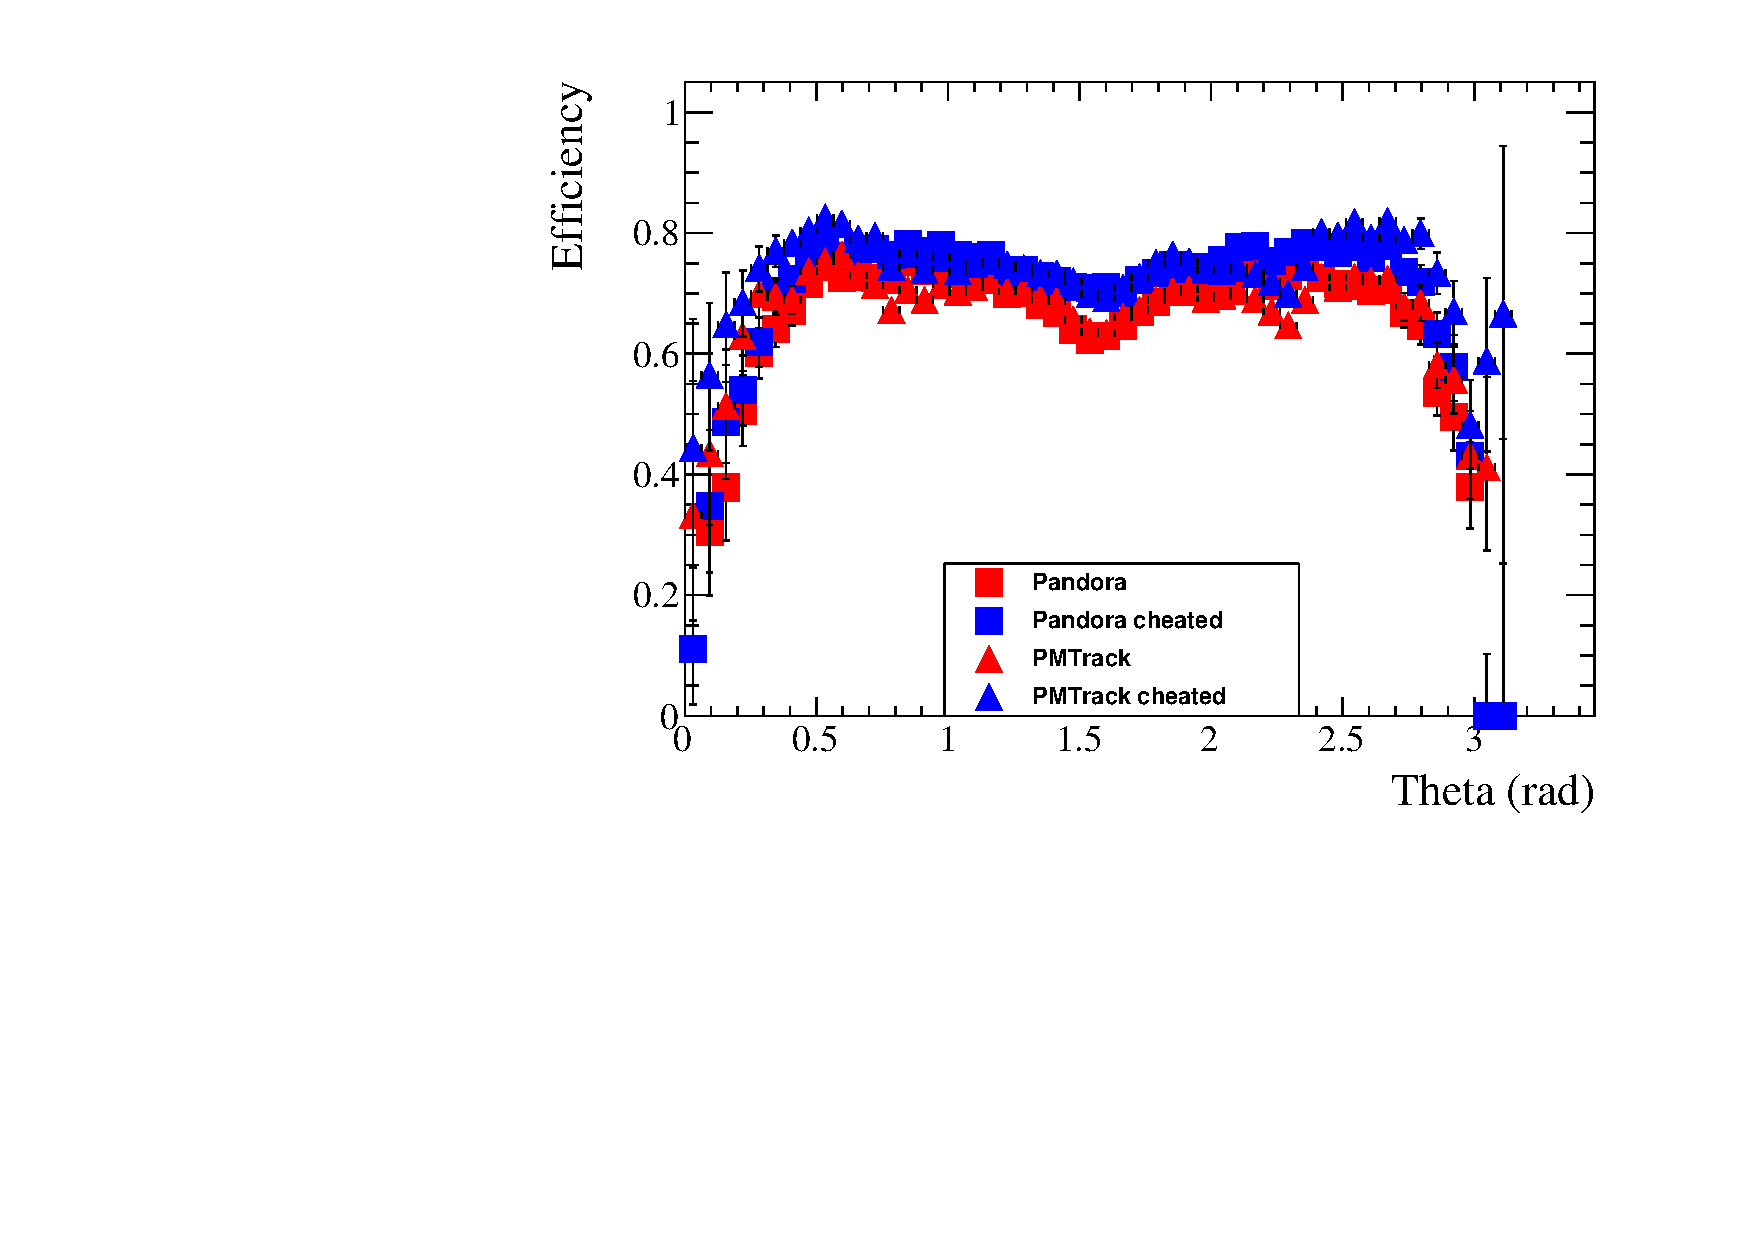
\includegraphics[width=\textwidth]{Effic_Cosmics_500V_All_Theta}
    \caption{Reconstruction efficiencies for a CRY sample.}
    \label{fig:SimEffic_Theta_CRY}
  \end{subfigure}
  \caption[The reconstruction efficiencies for simulated events as a function of Monte Carlo truth track angle in theta.]
          {The reconstruction efficiencies for simulated events as a function of Monte Carlo truth track angle in theta. The efficiencies are shown for non-cheated reconstruction (square blocks) and cheated reconstruction (triangle blocks) for both PMTrack (black) and Pandora (blue).}
          \label{fig:SimEffic_Theta}
\end{figure}

\begin{figure}[h!]
  \centering
  \begin{subfigure}{0.45\textwidth}
    \centering
    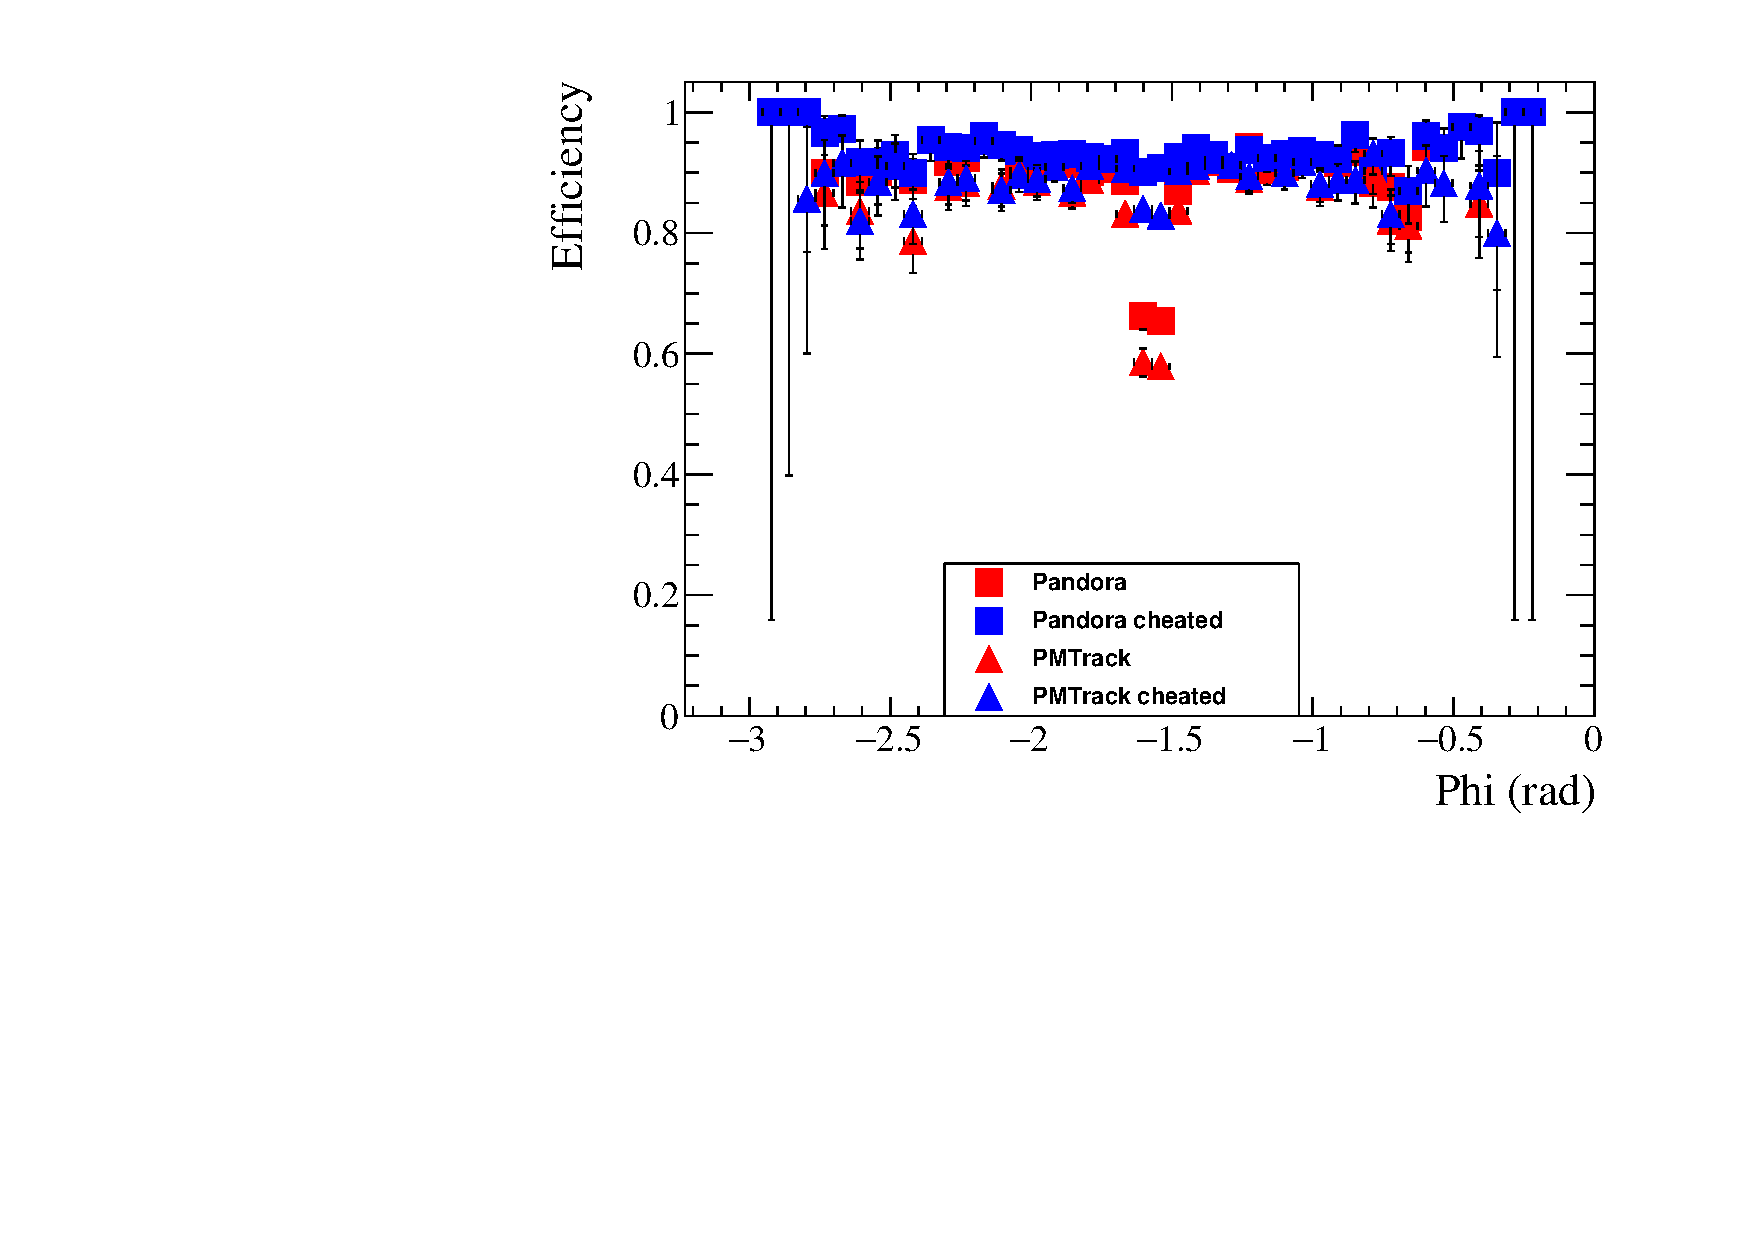
\includegraphics[width=\textwidth]{Effic_AntiMuon_500V_All_Phi}
    \caption{Reconstruction efficiencies for an Anti-Muon sample.}
    \label{fig:SimEffic_Phi_AMu}
  \end{subfigure}
  \hspace{0.08\textwidth}
  \begin{subfigure}{0.45\textwidth}
    \centering
    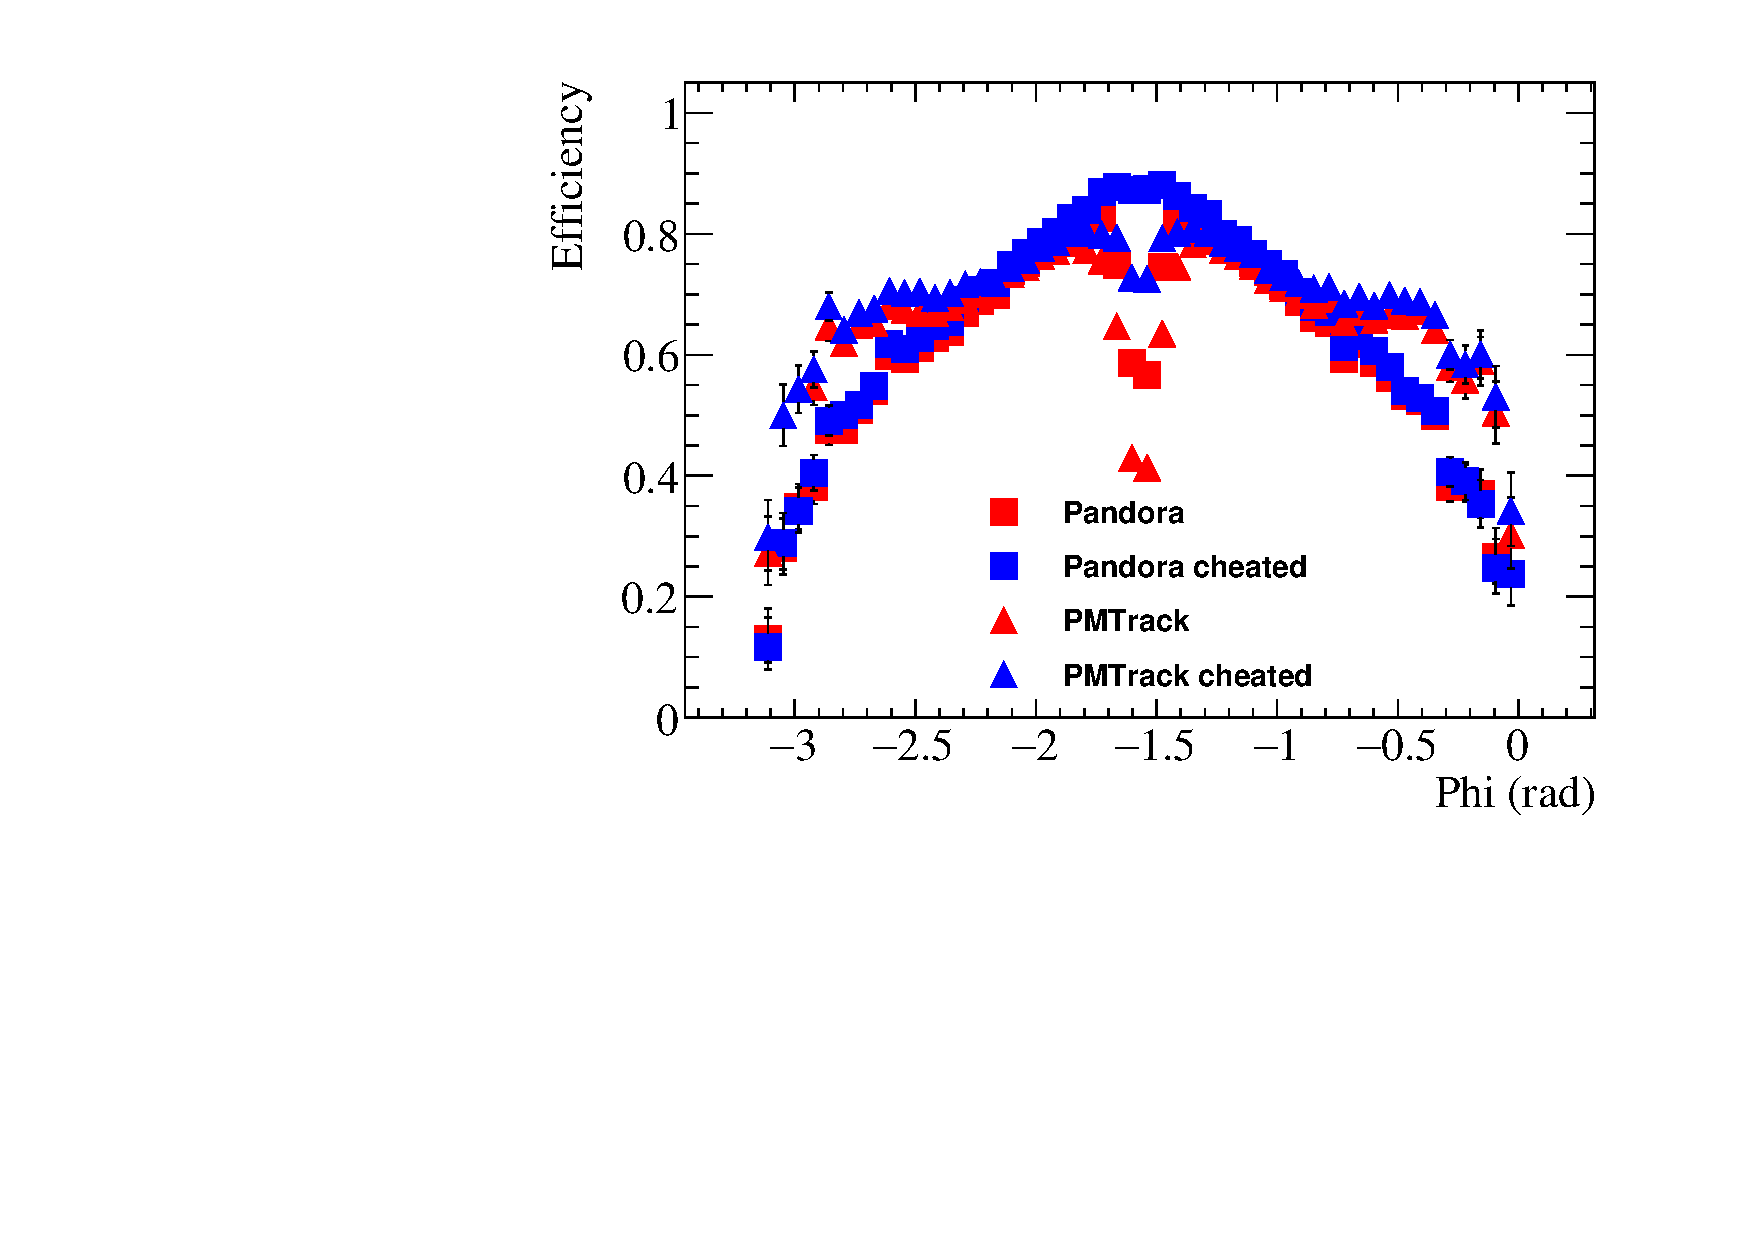
\includegraphics[width=\textwidth]{Effic_Cosmics_500V_All_Phi}
    \caption{Reconstruction efficiencies for a CRY sample.}
    \label{fig:SimEffic_Phi_CRY}
  \end{subfigure}
  \caption[The reconstruction efficiencies for simulated events as a function of Monte Carlo truth track angle in phi.]
          {The reconstruction efficiencies for simulated events as a function of Monte Carlo truth track angle in phi. The efficiencies are shown for non-cheated reconstruction (square blocks) and cheated reconstruction (triangle blocks) for both PMTrack (black) and Pandora (blue).}
          \label{fig:SimEffic_Phi}
\end{figure}

\begin{figure}[h!]
  \centering
  \begin{subfigure}{0.45\textwidth}
    \centering
    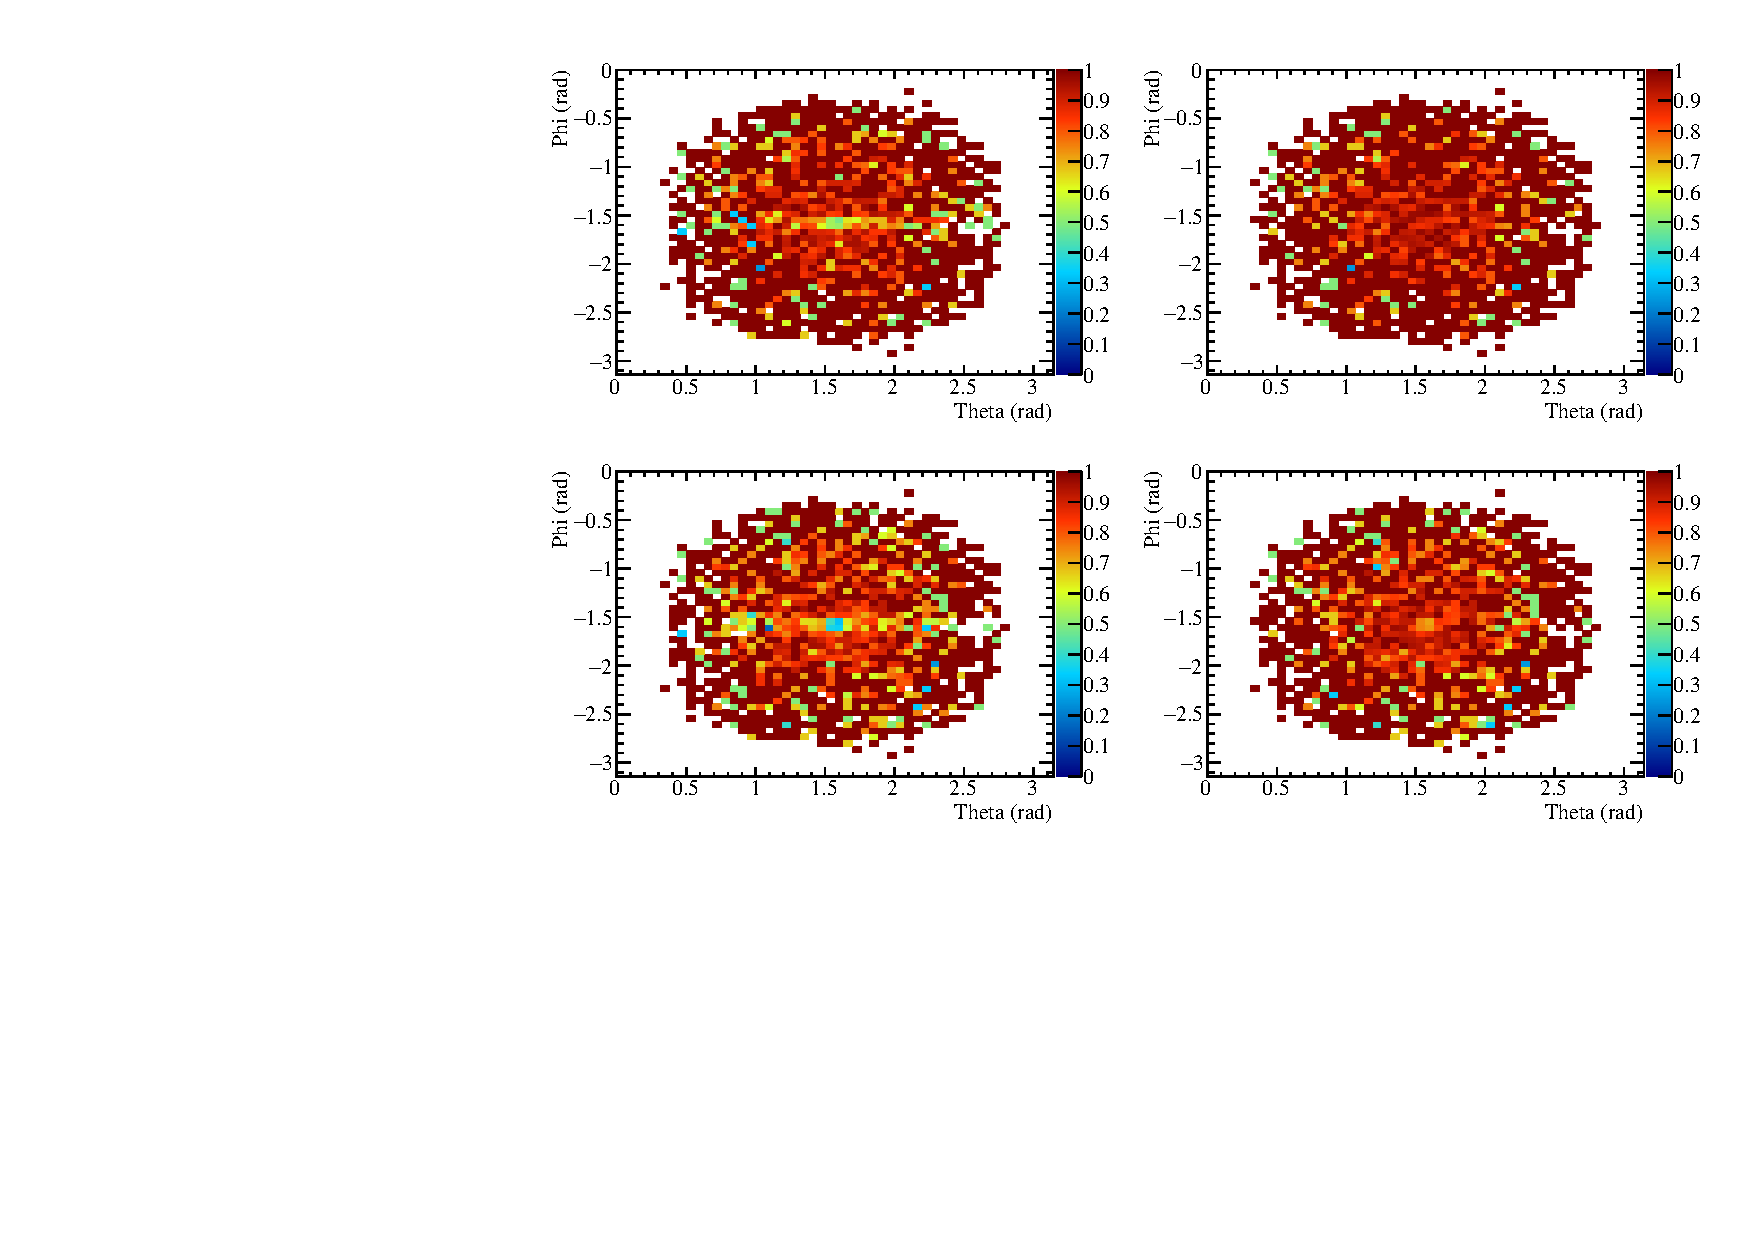
\includegraphics[width=\textwidth]{Effic_AntiMuon_500V_All_PhiTheta}
    \caption{Reconstruction efficiencies for an Anti-Muon sample.}
    \label{fig:SimEffic_ThetaPhi_AMu}
  \end{subfigure}
  \hspace{0.08\textwidth}
  \begin{subfigure}{0.45\textwidth}
    \centering
    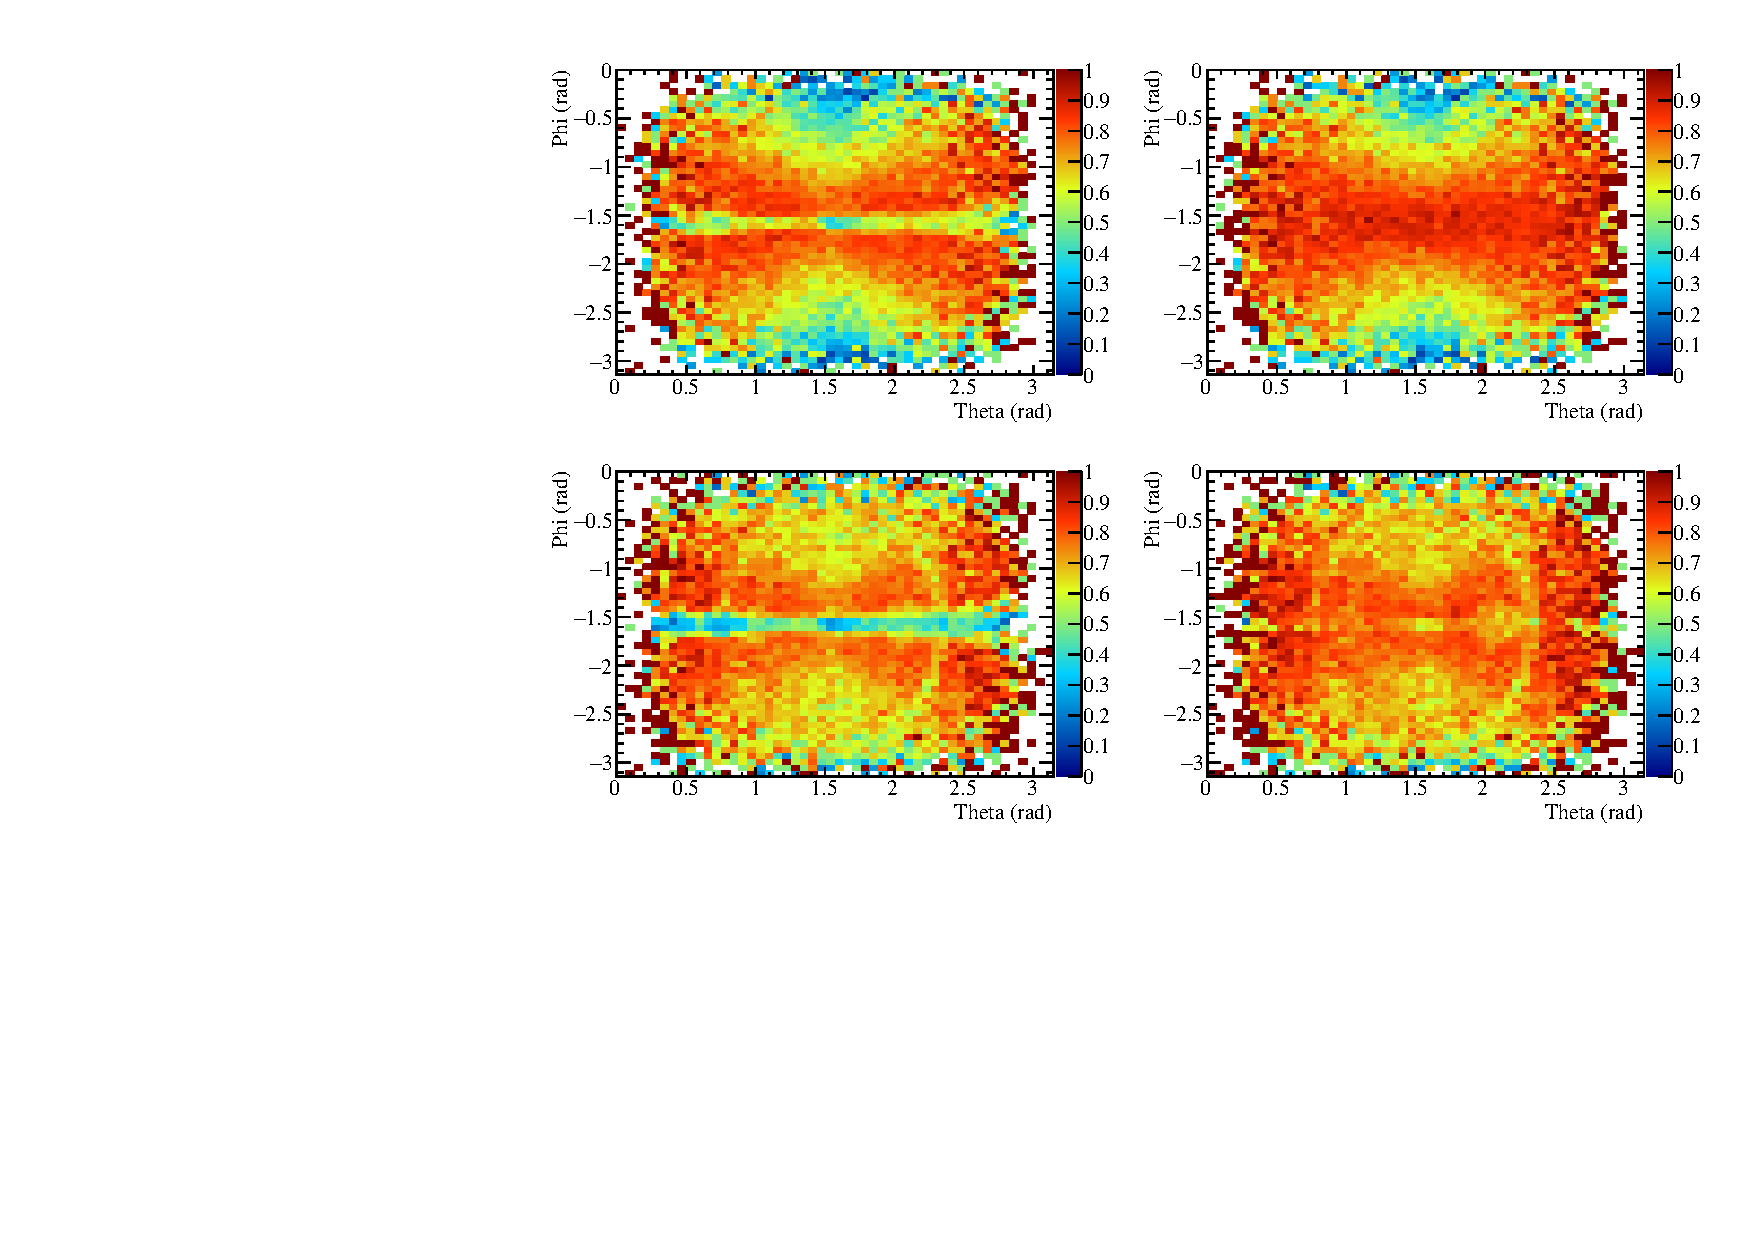
\includegraphics[width=\textwidth]{Effic_Cosmics_500V_All_PhiTheta}
    \caption{Reconstruction efficiencies for a CRY sample.}
    \label{fig:SimEffic_ThetaPhi_CRY}
  \end{subfigure}
  \caption[The reconstruction efficiencies for simulated events as a function of Monte Carlo truth track angle in theta and phi.]
          {The reconstruction efficiencies for simulated events as a function of Monte Carlo truth track angle in theta and phi. The efficiencies are shown for non-cheated reconstruction (plots on the left) and cheated reconstruction (plots on the right) for both Pandora (plots on the top) and PMTrack (plots on the bottom).}
          \label{fig:SimEffic_ThetaPhi}
\end{figure}

A striking feature of Figure~\ref{fig:SimEffic_Length} is the rapid decrease in reconstructed efficiency for the CRY sample for track lengths above 250 cm when using Pandora. The cause of this is that tracks are reconstructed separately in the long and short drift volumes before being merged when they are found to be co-linear in the $yz$ plane. This is not a problem in the Anti-Muon sample as the $x$ position of the hits calculated using Equation~\ref{eq:HitTime} will be correct. However, when the same is done for hits in the CRY sample using particles with large interaction times the $x$ positions will have offsets proportional to the interaction time unless the hit time is corrected by Equation~\ref{eq:HitTime_Int}. The result of this is that merged tracks can have discontinuities in their $x$ coordinates of more than 20 m. As the interaction time of the track is calculated using the output of the tracking algorithms it is not possible to directly correct for the interaction time at present. It is however possible to subtract this jump in $x$ position from the track length quantity which is calculated when the stitched track is stored in the event, this will give the correct track length though the user will still have to correct individual hit positions in later analyses using the calculated interaction time. This is what is done by PMTrack, hence it not exhibiting this rapid decrease in reconstruction efficiency for long tracks. \\

\begin{subequations} \begin{align}
  x_{Hit} &= T_{Hit} \times v_{Drift} \label{eq:HitTime} \\
  T_{Hit} &= T_{Measured} - T_{Interaction} \label{eq:HitTime_Int}
\end{align} \end{subequations}

It is clear from Figure~\ref{fig:SimEffic_Length} that tracks of lengths less than 30 cm are poorly reconstructed. The very low efficiency for tracks of less than 10 cm can be partially attributed to particles of lengths less than 1 cm as these particles are too short to be reconstructed using the current reconstruction process. These very short particles represent ~30\% of the particles with lengths below 10 cm. Though these particles will need to be reconstructed when looking for supernovea bursts special algorithms will probably be written as these particles will only cross 1 or 2 wires in each plane and so may look similar to noise hits meaning that they will not be combined into clusters. Another issue is that the low energies of these particles may mean that the hits are below threshold and so will not be reconstructed. The reconstruction of longer tracks will also be affected by the number of wires which they cross, though this should matter much less for particles with lengths of more than 5 cm as they will have crossed roughly 10 wires in each plane, this should be enough to reliably construct clusters. This can be seen to be the case for PMTrack when considering the Anti-Muon sample, as the efficiencies for track lengths between 10 and 20 cm is roughly the same as that for track lengths between 20 and 30 cm, however when considering the CRY sample there is still a significant decrease in efficiency. This is attributed to the more complex event structure in the CRY sample, where secondary particles are produced which are mis-reconstructed, as when considering only muons the reconstruction efficiency is seen to be the same as that for the Anti-Muon sample. \\

The trend of increasing efficiency for longer track lengths from Figure~\ref{fig:SimEffic_Length} can also be seen in Figure~\ref{fig:SimEffic_EnDepos} as the energy deposited increases. This is because particles which deposit more energy will tend to have travel further in the detector. The amount of energy that paticles deposit is limited by the size of the detector though as particles with an energy of more than 1 GeV are energetic enough to through-going MIPS. This results in few particles depositing more than 1 GeV in the detector causing the uncertainty in the reconstrution efficiency to increase above this energy. \\

It is also interesting to note the pronounced decreases in reconstruction efficiencies for particular angles shown in Figure~\ref{fig:SimEffic_Theta} and Figure~\ref{fig:SimEffic_Phi}. The decrease in efficiency at $\phi = \frac{\pi}{2}$ can be attributed to the drop in efficiency for tracks of ~200 cm, as this corresponds to the vertical height of the detector meaning that few colletion wires are hit and so determining the triple points needed by the disambiguation are difficult to find. This is verified by the large increase in efficiency achieved by cheating the disambiguation. Similarly the decrease in efficiency at $\theta = \frac{\pi}{2}$ can be attributed to particles which are perpendicular to the collection wires resulting in few collection wires being hit. \\  

The information from Figures~\ref{fig:SimEffic_Theta} and~\ref{fig:SimEffic_Phi} is combined in Figure~\ref{fig:SimEffic_ThetaPhi} where the sharp drops in efficiency for the CRY sample are particularly visible. The effect of cheated disambiguation is clear in Figure~\ref{fig:SimEffic_ThetaPhi_CRY} where the dip in efficiency as a function of $\theta$ at fixed $\phi=\frac{\pi}{2}$ is completely removed. The same is not true for the dip in efficiency as a funciton $\phi$ at fixed $\theta = \frac{\pi}{2}$, though the reduction in efficiency was not uniform or as severe across all values of $\theta$ as it remains mainly confined to values of $\theta$ close to 0 or $\pi$, particularly when using Pandora . The observation that a significant improvement in the quality of reconstruction can be made in improving the disambiguation is a driving force in the wire pitches being 36$^{\circ}$ for the DUNE FD as opposed 45$\pm$0.7$^{\circ}$ in the 35 ton, because as discussed in Section~\ref{sec:LArSoft} the shallower wire pitch makes disambiguation easier. Though disambiguation will be easier in the different geometry, further efforts to improve disambiguation are still required, as are continued efforts to reconstruct the shortest tracks. \\

%********************************** % Fourth Section  *************************************
\section{Performing particle identification}  %Section - X.4
Being able to perform reliable particle identification (PID) is key deliverable for the DUNE experiment, and so efforts have been made to establish a metric by which this can be achieved. The predominant method of performing PID in LAr is to use the relationship between $\frac{dE}{dx}$ and the residiual range of the track, defined as being the distance between a point on the track and the stopping point of the track. The relationship between these particle is observed to be dependent on particle mass and is quantified by the Bethe-Bloch equation!!!citep{BetheBloch}!!! which is shown in Figure~\ref{fig:BetheBloch}. The sharp increase in energy loss per unit length can be seen to occur at different momenta for different particle masses meaning that the peak value of $\frac{dE}{dx}$ can change significantly. One example of a large change in the peak value of $\frac{dE}{dx}$ can be seen by comparing muons and protons, whist muons and pions are very similar. \\

\begin{figure}[h!]
  \centering
  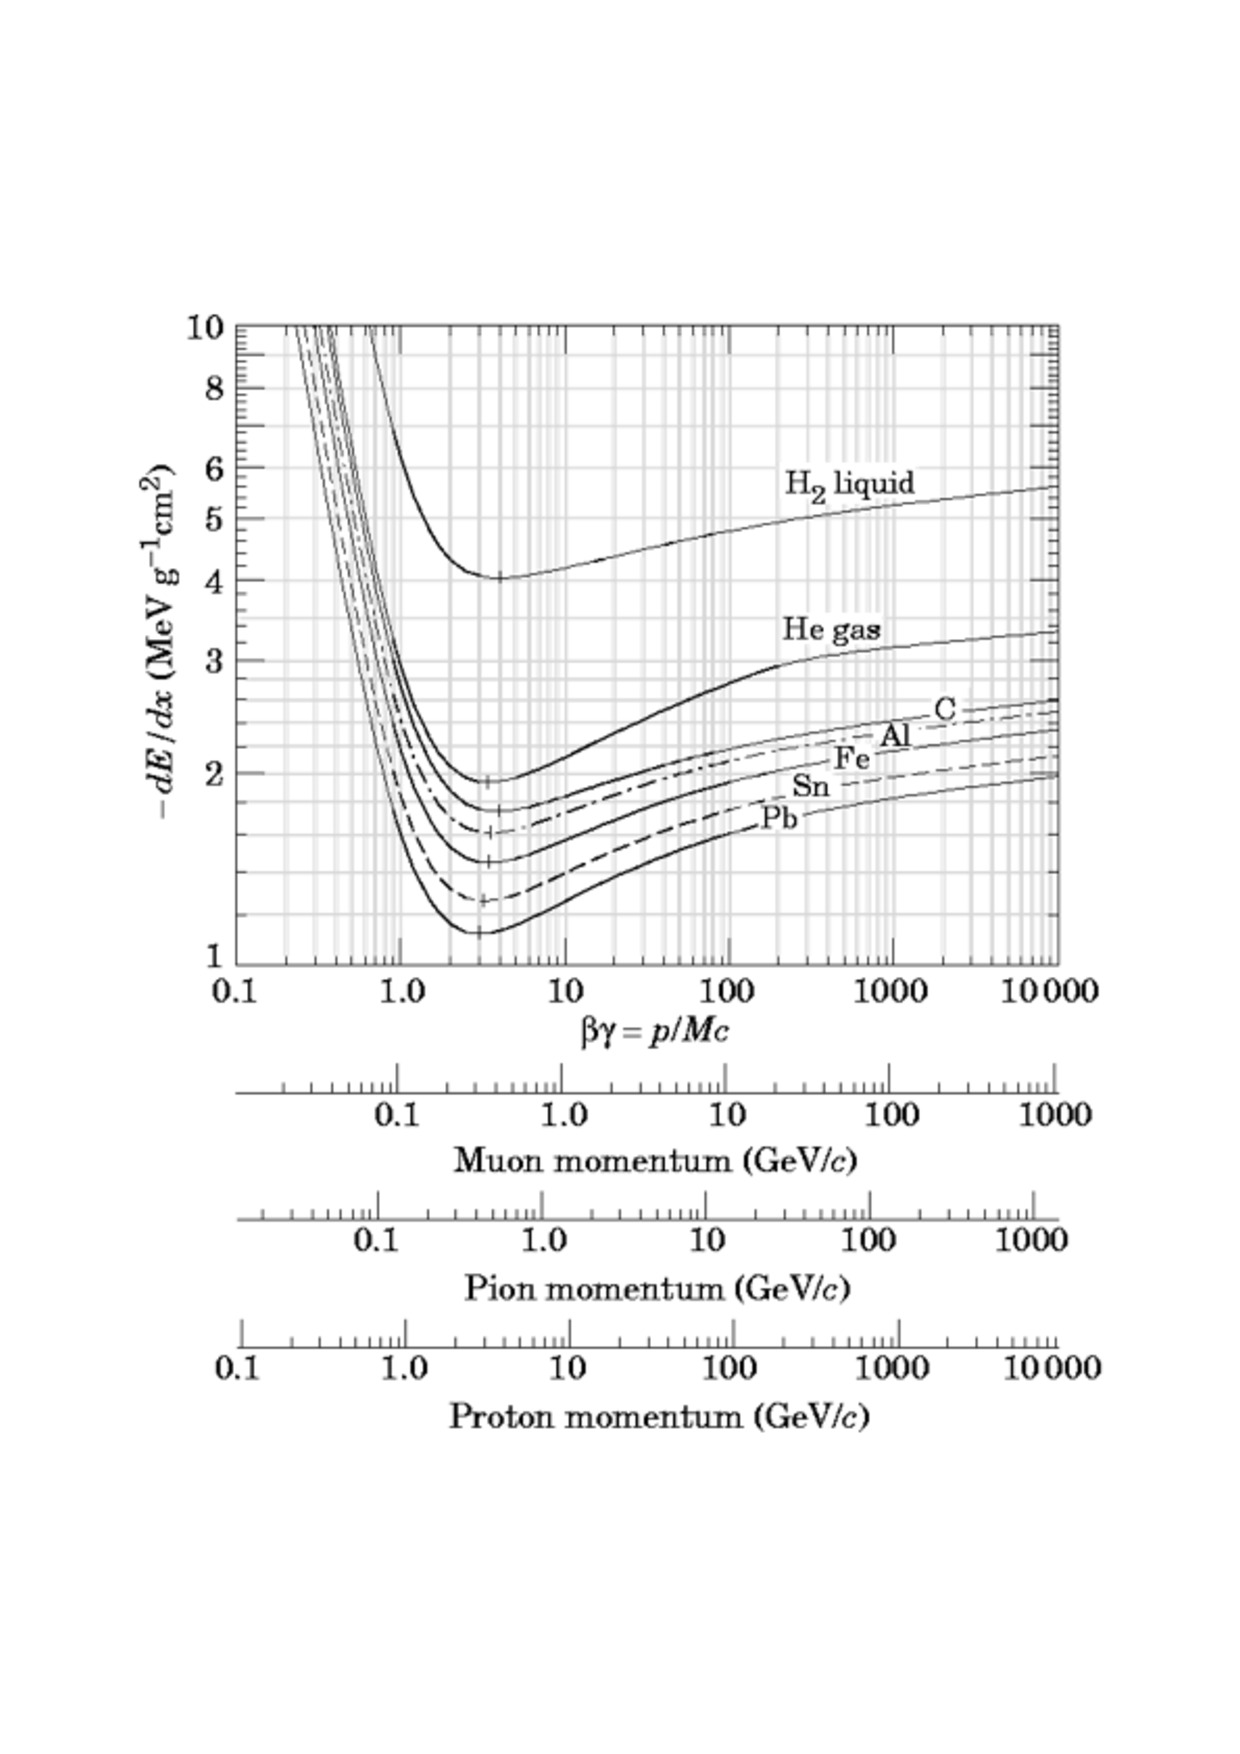
\includegraphics[width=0.5\textwidth]{BetheBlock}
  \caption[The medium and particle type dependence of the Bethe-Bloch equation]
          {The Bethe-Bloch equation describes energy loss per unit length as a function of energy in different mediums. The energy losses expected for different particle types is shown in different mediums. Liquid Argon with a density of 1.4 g cm$^{-3}$ has a density slightly less than that of Carbon at 1.8 g cm$^{-3}$.}
  \label{fig:BetheBloch}
\end{figure}

The particle mass dependance can be seen by plotting the $\frac{dE}{dx}$ against the residiual range of the particle on a log-log plot, as shown in Figure~\ref{fig:PIDA_loglog}. A power law dependence is found to describe the relationship~\citep{PIDA_Paper}, as shown in Equation~\ref{eq:PIDA}. The dependence on $b$ is found to be weak, and so can be set to -0.42 for all particle masses. This means that the main discriminant used is the $A$ parameter, which has a strong dependence on particle mass. The values for $A$ and $b$ calculated from Figure~\ref{fig:PIDA_loglog} are shown in Table~\ref{tab:PIDAVals}. It is found that the error introduced by fixing the $b$ parameter is small compared to the error from ionization fluctuations. \\

Once the $b$ parameter is set to be constant for all particle types it is possible to calculate a value for the $A$ parameter for each hit on the track using Equation~\ref{eq:PIDA_A}, where $R_i$ is the residual range of the track at that point. The particle type discriminant, called PIDA, can then be calculated for a track by finding the average value of $A_i$ found for the track. As the particle mass dependant increase in $\frac{dE}{dx}$ only occurs near the end of the track, the PIDA variable can only be calculated for particles which stop in the detector as all other particles will have MIP-like $\frac{dE}{dx}$ distributions and so cannot be identified in this way. As shown by the plotted range of Figure~\ref{fig:PIDA_loglog} the average value of $A$ is normally calculated for the last 30 cm of the track. \\

\begin{equation}
  \label{eq:PIDA}
  \frac{dE}{dx}_{calo} = A R^b
\end{equation}

\begin{equation}
  \label{eq:PIDA_A}
  A_i = (\frac{dE}{dx}_{calo})_i \times R^{0.42}_i
\end{equation}

The PIDA method was tested in~\citep{PIDA_Paper}, where the PIDA values were calculated for Monte Carlo particles which stopped in the detector using truth information over the last 30 cm of the particle lengths. This is shown in Figure~\ref{fig:PIDA_MC}, where a clear separation can be seen between the peaks for Muons, Pions, Kaons and Protons. Though the Muon and Pion peaks are relatively close together they can still be resolved in the plot due to little overlap. It is interesting to note how tight the PIDA distributions found in the paper are, which allows the different particles types to cleanly separated in the truth study. The author notes that an incorrect tuning of the recombination effects will cause the distributions to become broader, and an incorrect calibration of the detector will introduce a systematic shift in the expected values of PIDA. \\

\begin{figure}[h!]
  \centering
  \begin{subfigure}{0.45\textwidth}
    \centering
    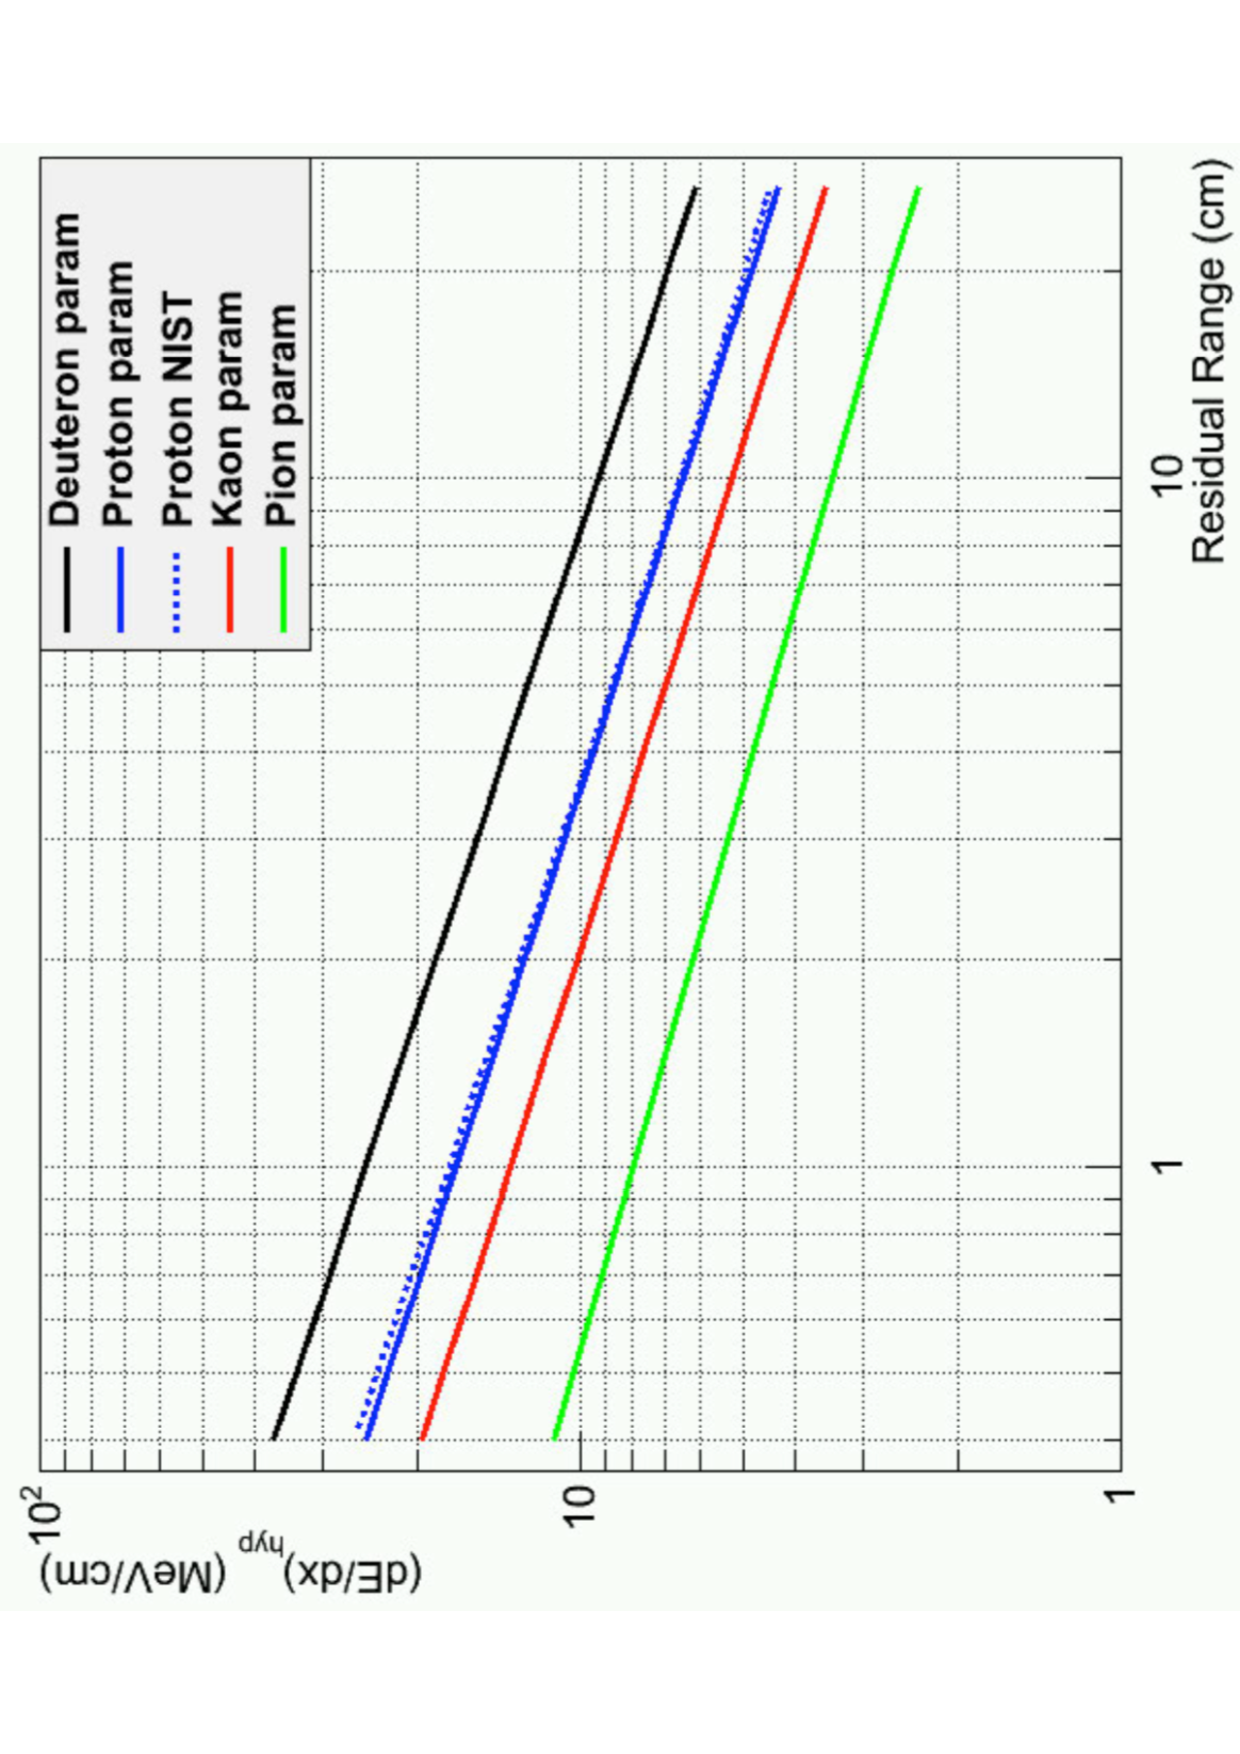
\includegraphics[width=\textwidth]{StoppingPower}
    \caption{Stopping power for different particle masses.}
    \label{fig:PIDA_loglog}
  \end{subfigure}
  \hspace{0.08\textwidth}
  \begin{subfigure}{0.45\textwidth}
    \centering
    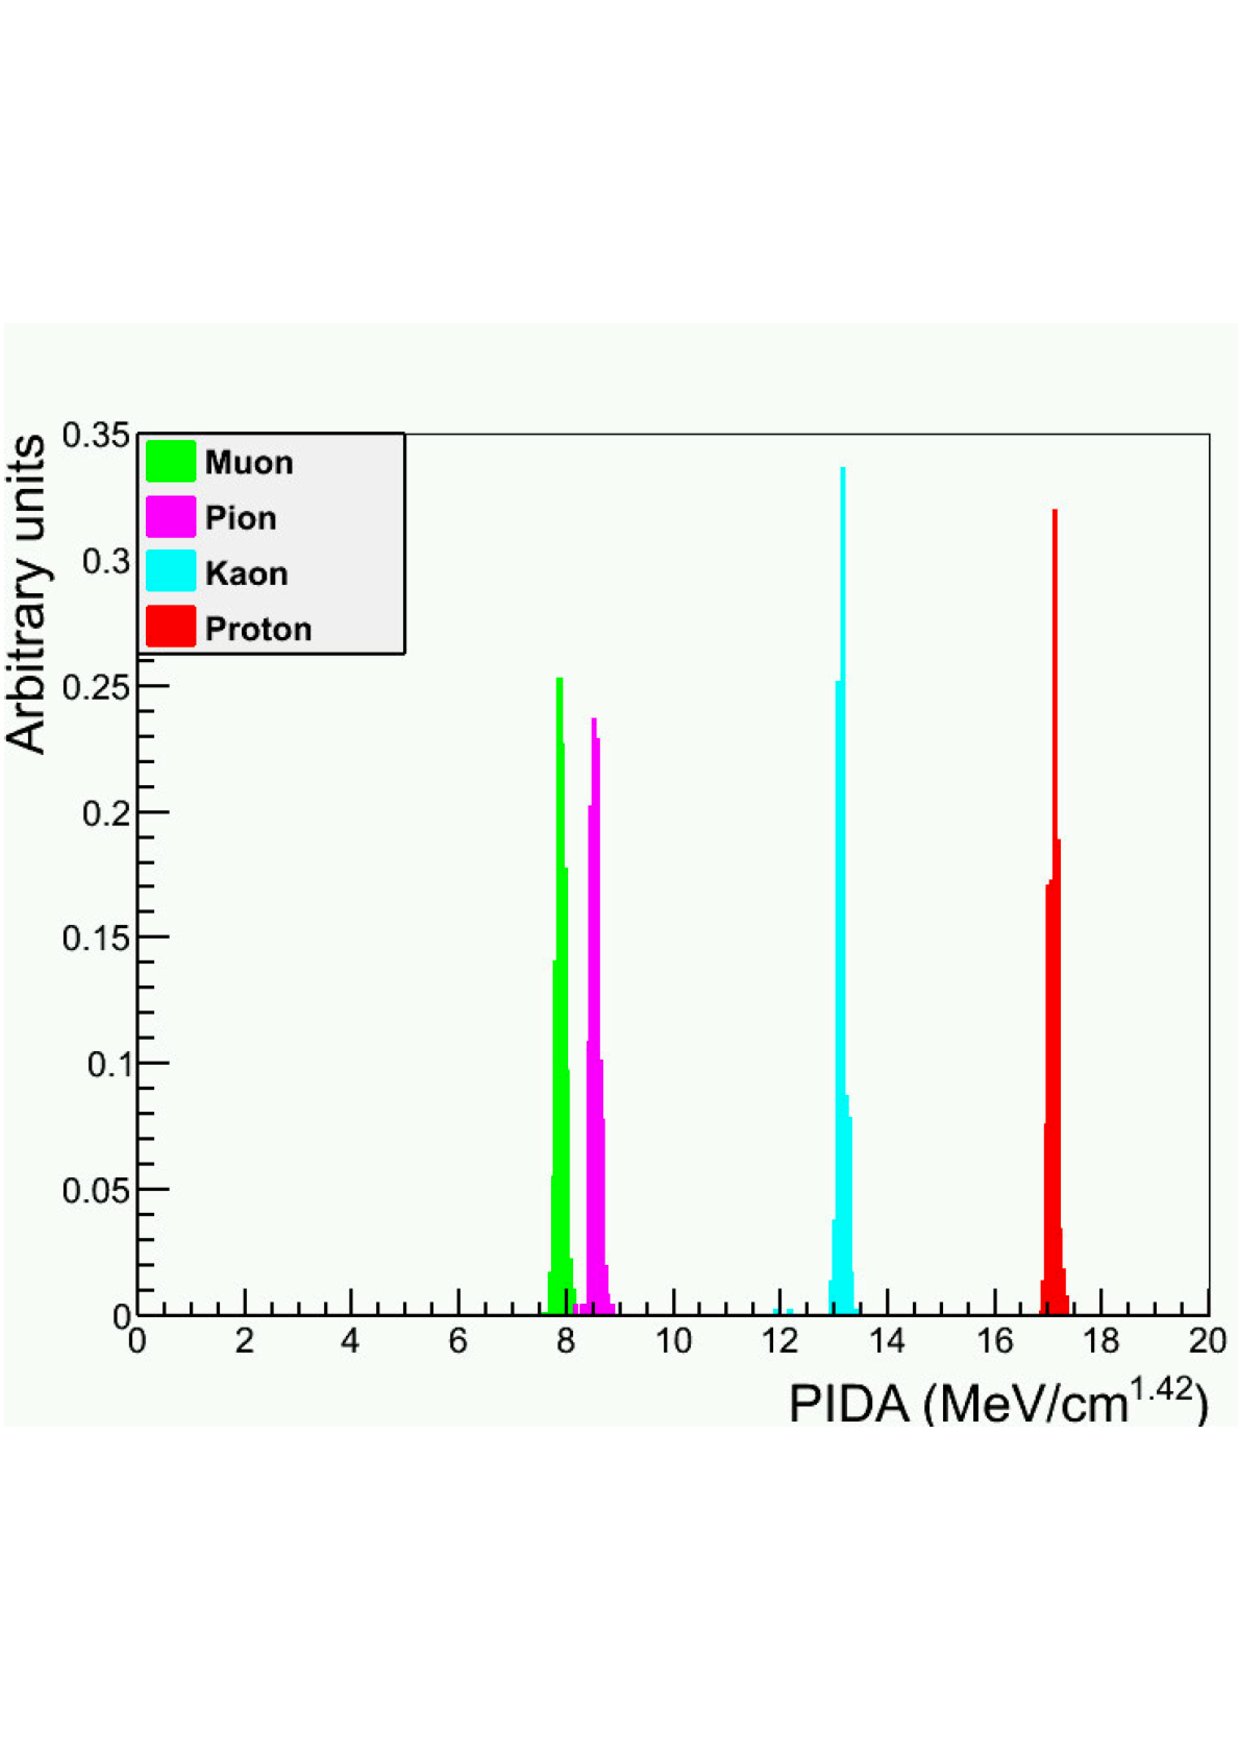
\includegraphics[width=\textwidth]{TruthPIDA}
    \caption{Distribution of PIDA values for different particle masses.}
    \label{fig:PIDA_MC}
  \end{subfigure}
  \caption[Defining the PIDA metric for particle identification.]
          {Defining the PIDA metric for particle identification and testing it on a Monte Carlo sample using truth information.}
          \label{fig:PIDAPlots}
\end{figure}

From Figure~\ref{fig:PIDAPlots} it can be seen that the most distinct PIDA distributions are that of muons and protons, these are also two of the most common particle types in cosmic rays. For these reasons particle identification using the PIDA varaible will be attempted on simulations of the 35 ton. As outlined in Sections~\ref{sec:SimInteractionTimes} and ~\ref{sec:MCCalib} in order to do this the interaction times of particles have to be well known and the calibration constants must be tuned so as to ensure that the effects of recombination are properly accounted for. It is also useful to use the information found in Section~\ref{sec:SimRecoEffic} about the efficiency with which tracks are reconstructed. In this regard it is useful to produce additional figures showing the reconstruction efficiencies of protons in the CRY sample, these are shown in Figure~\ref{Prot_Effic}.\\

\begin{figure}[h!]
  \centering
  \begin{subfigure}{.45\textwidth}
        \centering
        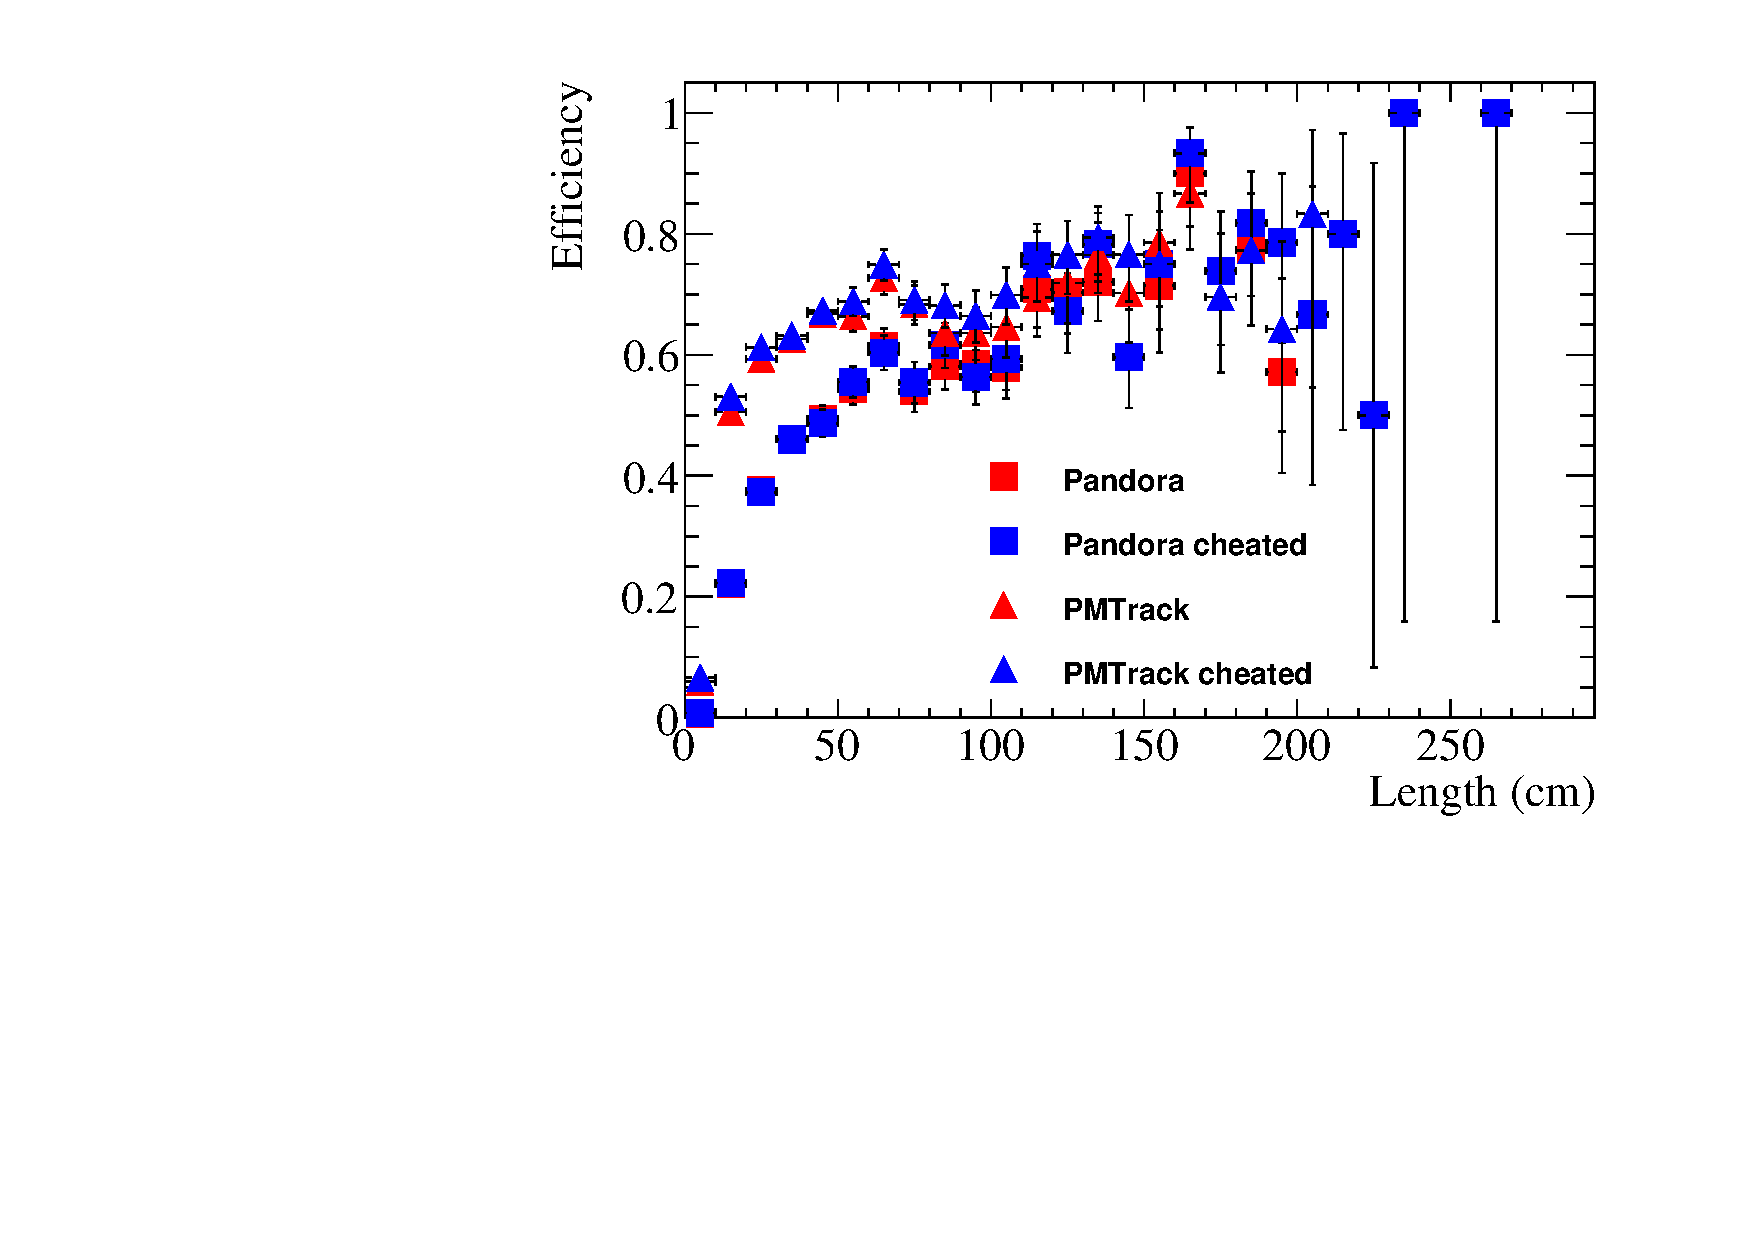
\includegraphics[width=\textwidth]{Effic_ProtonEnrich_500V_Proton_Length}
        \caption{The reconstruction efficiency as a function of Monte Carlo truth track length.}
        \label{fig:Prot_Effic_Len}
  \end{subfigure}
  \hspace{0.08\textwidth}
  \begin{subfigure}{.45\textwidth}
        \centering
        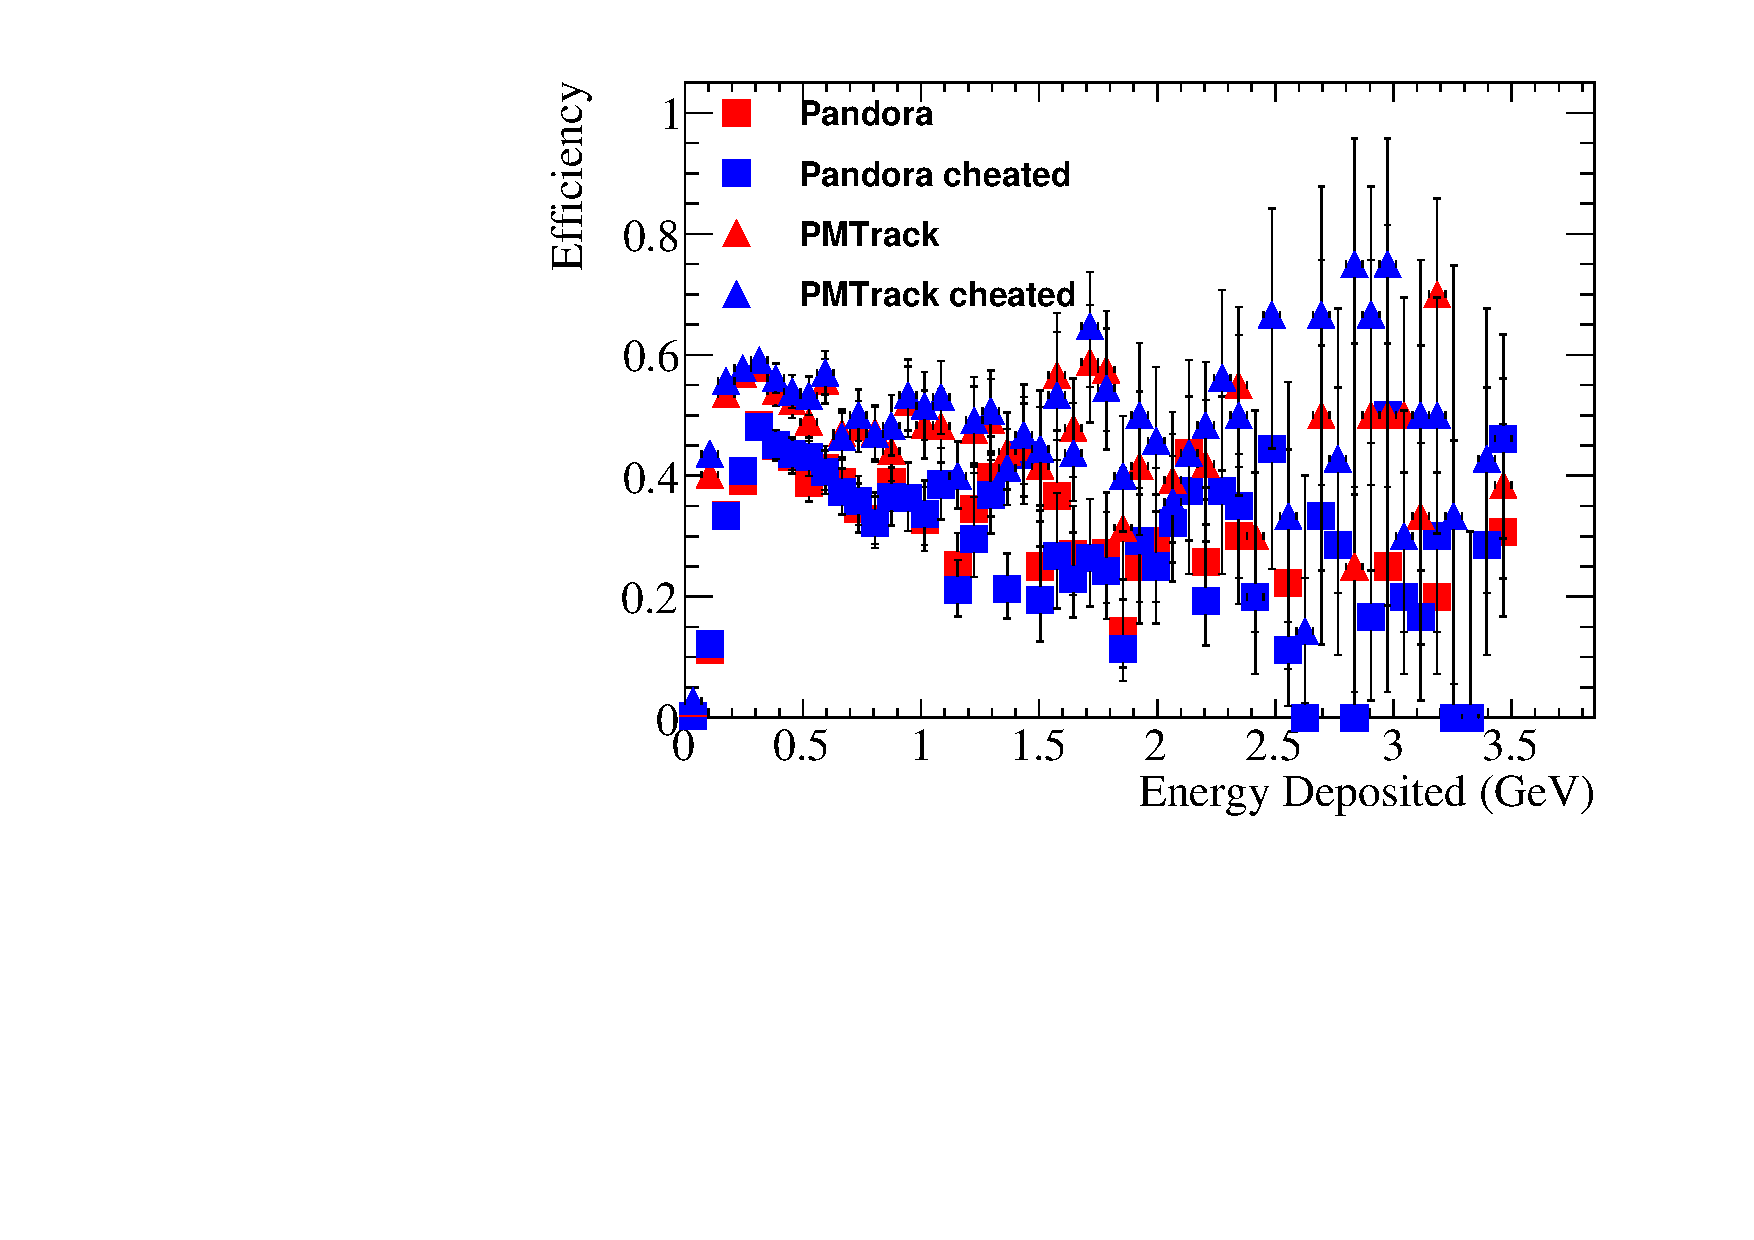
\includegraphics[width=\textwidth]{Effic_ProtonEnrich_500V_Proton_EnDepos}
        \caption{The reconstruction efficiency as a function of Monte Carlo truth deposited energy.}
        \label{fig:Prot_Effic_EnDepos}
  \end{subfigure}
  \begin{subfigure}{.45\textwidth}
        \centering
        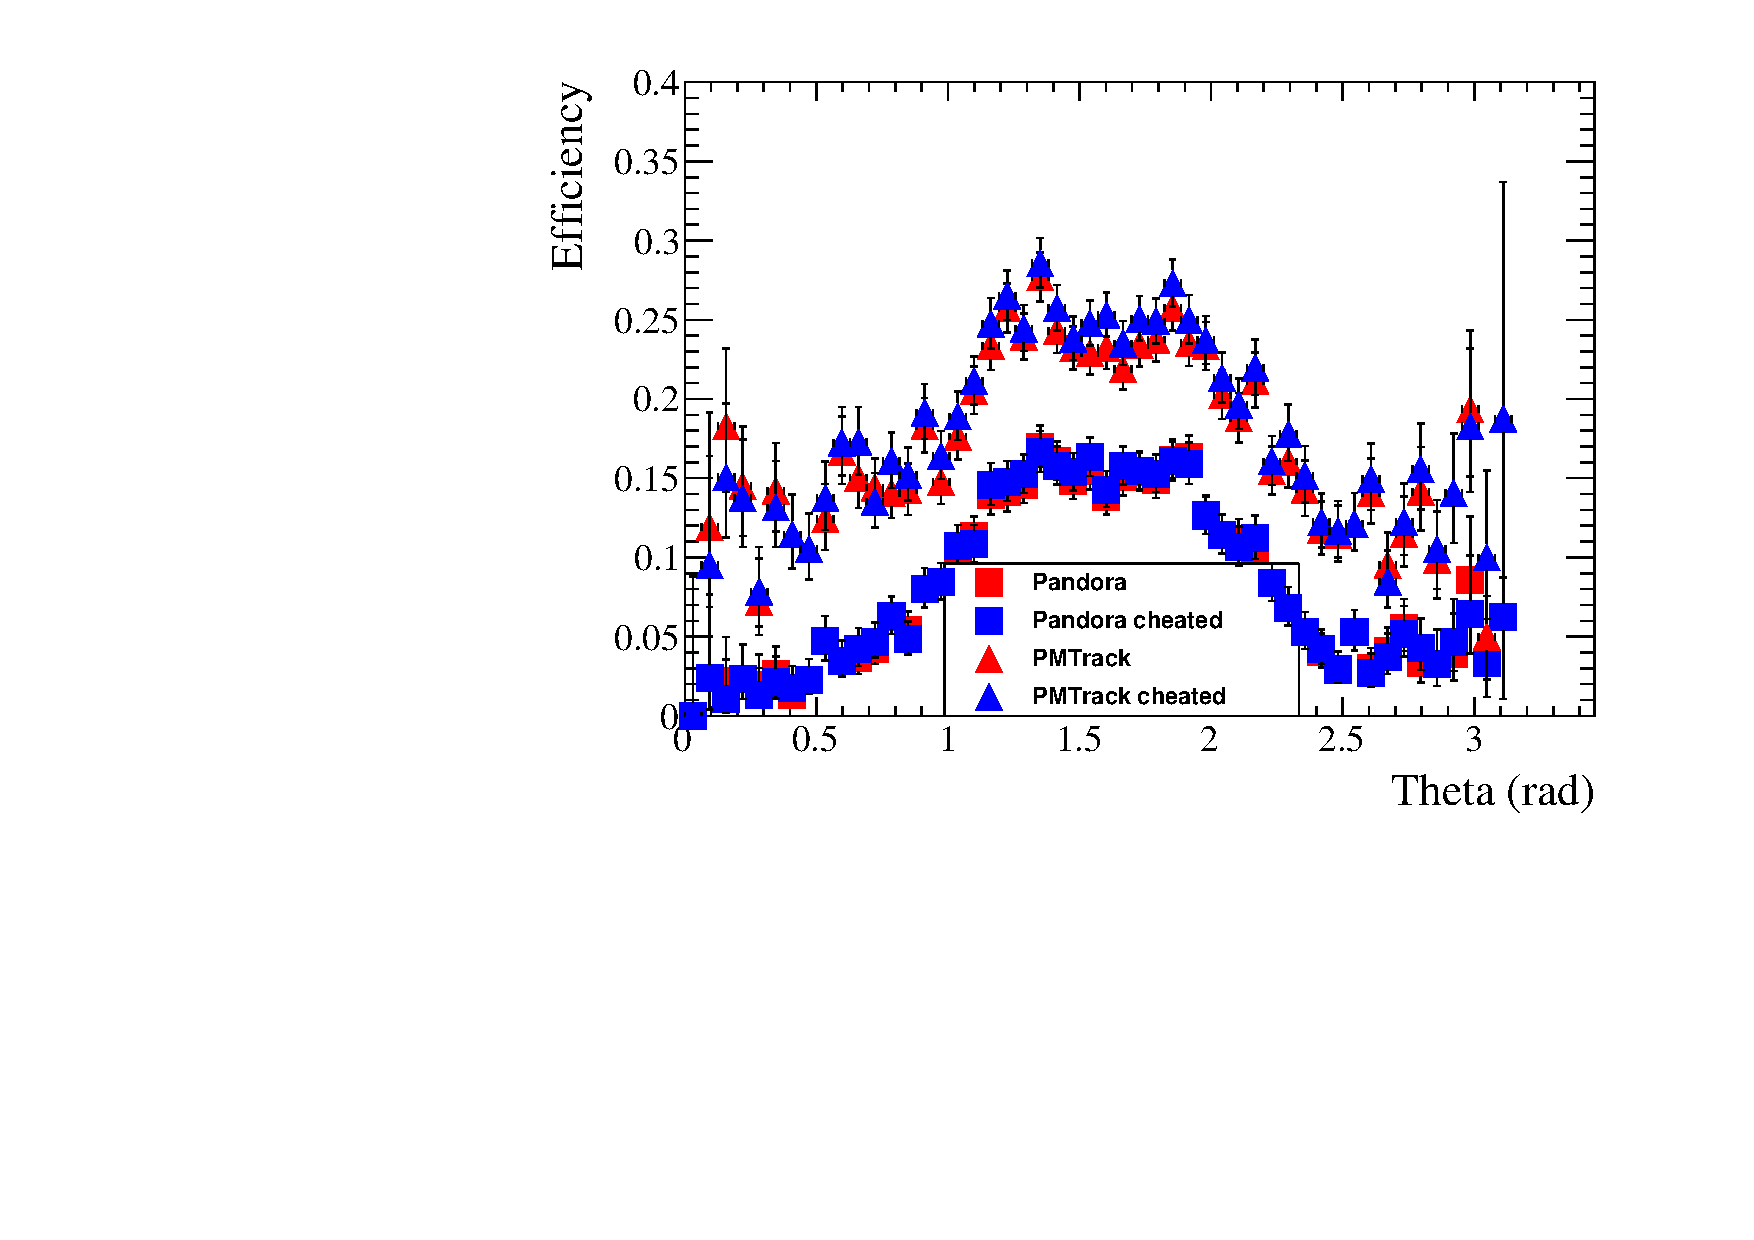
\includegraphics[width=\textwidth]{Effic_ProtonEnrich_500V_Proton_Theta}
        \caption{The reconstruction efficiency as a function of Monte Carlo truth track angle in theta.}
        \label{fig:Prot_Effic_Theta}
  \end{subfigure}
  \hspace{0.08\textwidth}
  \begin{subfigure}{.45\textwidth}
        \centering
        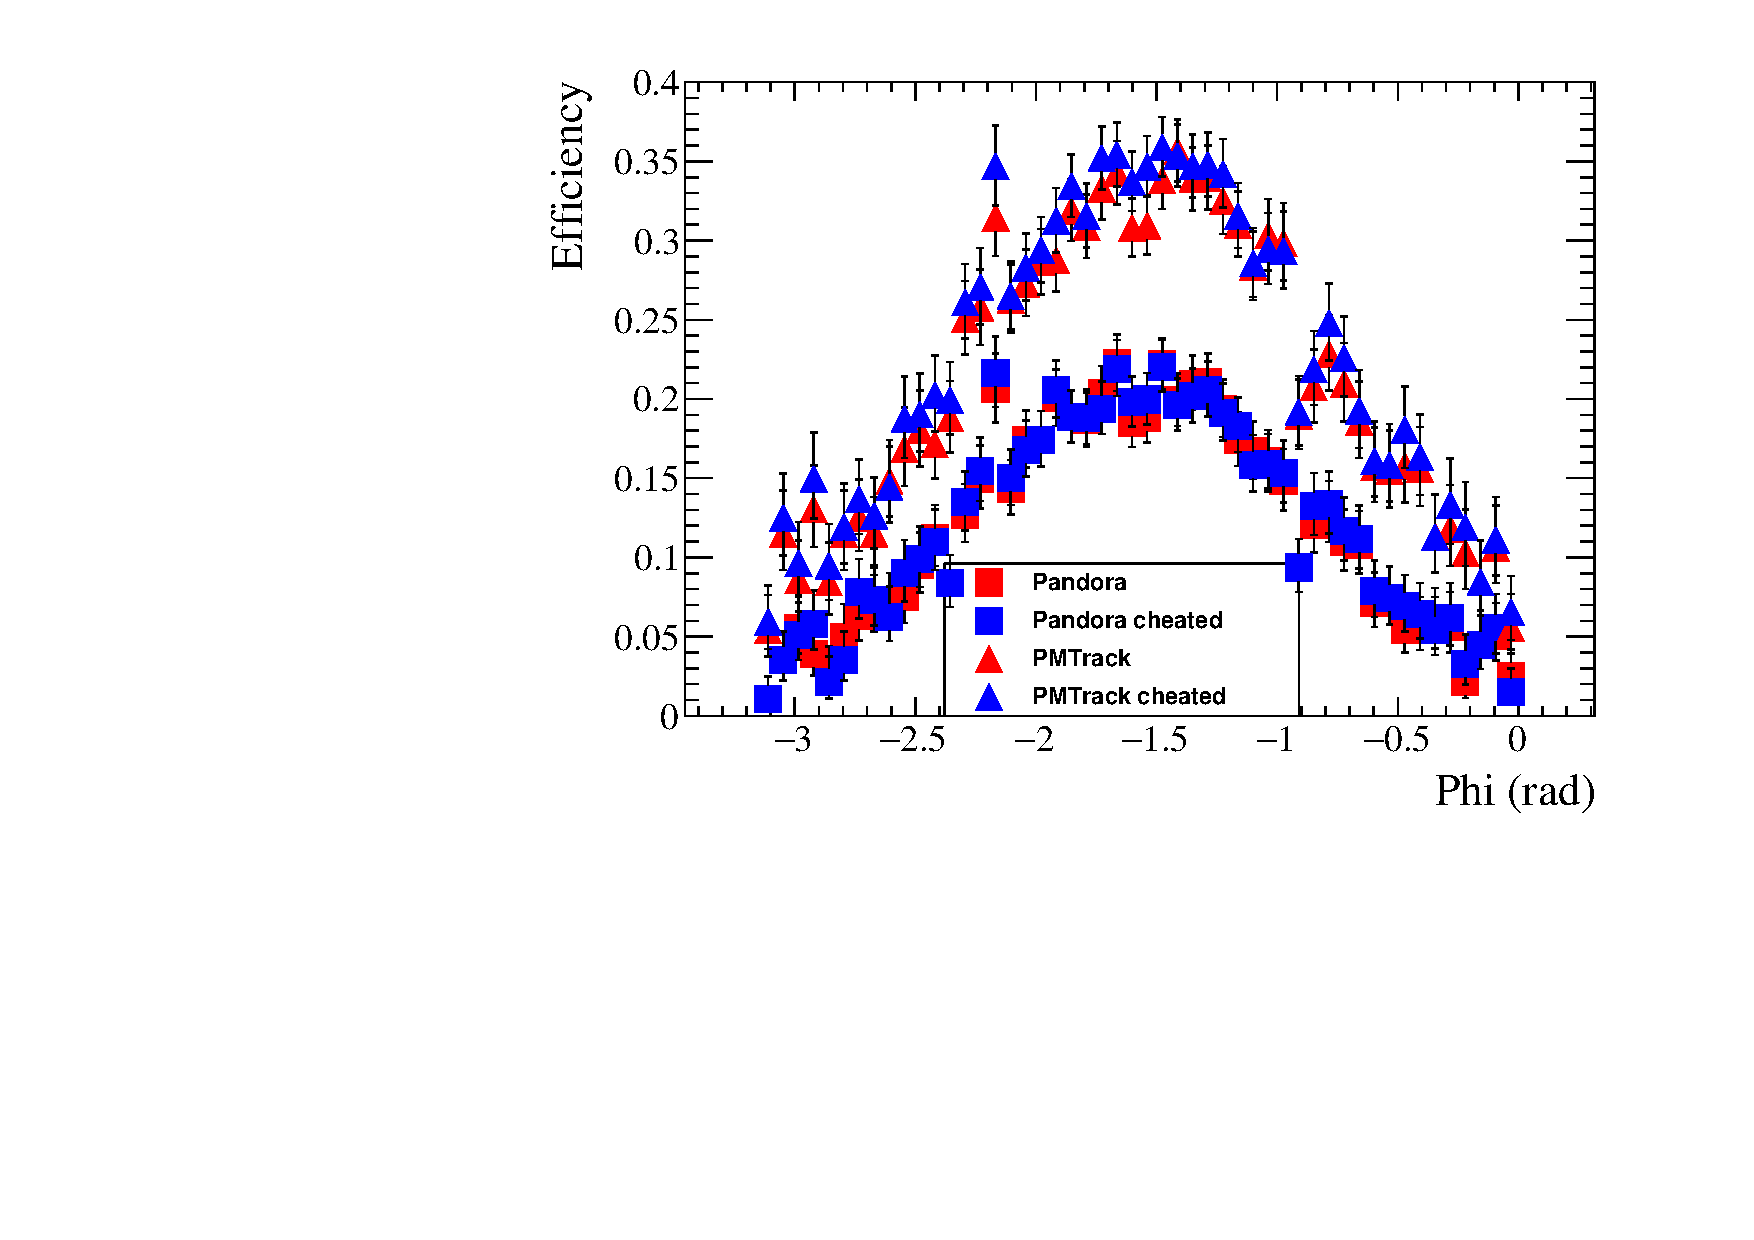
\includegraphics[width=\textwidth]{Effic_ProtonEnrich_500V_Proton_Phi}
        \caption{The reconstruction efficiency as a function of Monte Carlo truth track angle in phi.}
        \label{fig:Prot_Effic_Phi}
  \end{subfigure}
  \begin{subfigure}{.45\textwidth}
        \centering
        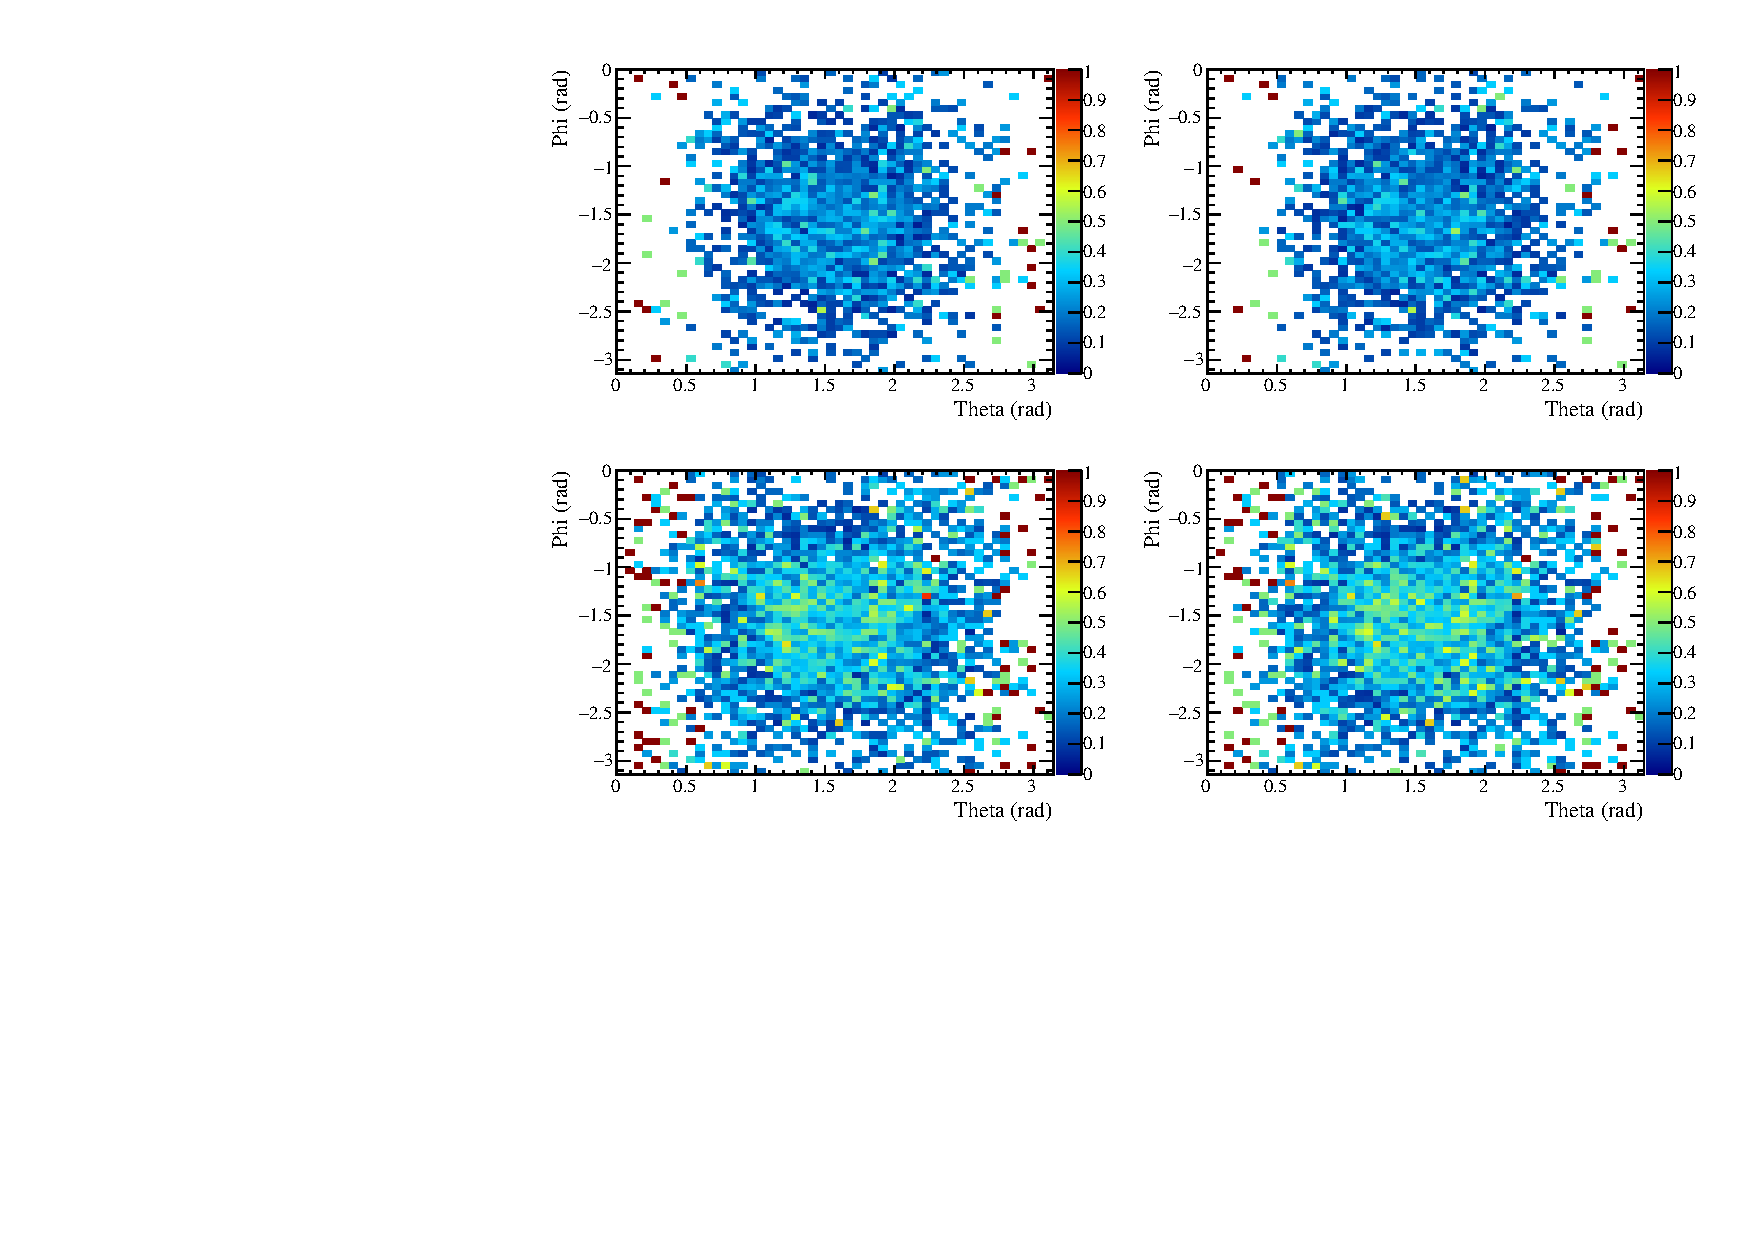
\includegraphics[width=\textwidth]{Effic_ProtonEnrich_500V_Proton_PhiTheta}
        \caption{The reconstruction efficiency as a function of Monte Carlo truth track angle in theta and phi.}
        \label{fig:Prot_Effic_PhiTheta}
  \end{subfigure}
  \caption[The reconstruction efficiencies for protons in a sample generated using CRY.]
          {The reconstruction efficiencies for protons in a sample generated using CRY. The efficiencies are shown for non-cheated reconstruction (square blocks) and cheated reconstruction (triangle blocks) for both PMTrack (black) and Pandora (blue).}
  \label{fig:Prot_Effic}
\end{figure}
